\documentclass[11pt]{report}
\usepackage{./assignment_programming}
\usepackage{slashbox}
%\usepackage{enumitem}
%\usepackage{stmaryrd}
%\usepackage{cprotect}
\usepackage{graphicx}
\usepackage{subfigure}

\RequirePackage{latexsym}
\RequirePackage{amsmath}
\RequirePackage{amssymb}
\RequirePackage{bm}
\RequirePackage{url}
\RequirePackage{algorithmic}
\RequirePackage{algorithm2e}


%%%%%%%% Stock standard definitions %%%%%%%%%%%%%%%

%\newcommand{\ab}{\mathbf{a}}
%\newcommand{\bb}{\mathbf{b}}
%\newcommand{\cbb}{\mathbf{c}}
%\newcommand{\db}{\mathbf{d}}
%\newcommand{\eb}{\mathbf{e}}
%\newcommand{\fb}{\mathbf{f}}
%\newcommand{\gb}{\mathbf{g}}
%\newcommand{\hb}{\mathbf{h}}
%\newcommand{\ib}{\mathbf{i}}
%\newcommand{\jb}{\mathbf{j}}
%\newcommand{\kb}{\mathbf{k}}
%\newcommand{\lb}{\mathbf{l}}
%\newcommand{\mb}{\mathbf{m}}
%\newcommand{\nbb}{\mathbf{n}}
%\newcommand{\ob}{\mathbf{o}}
%\newcommand{\pb}{\mathbf{p}}
%\newcommand{\qb}{\mathbf{q}}
%\newcommand{\rb}{\mathbf{r}}
%\newcommand{\sbb}{\mathbf{s}}
%\newcommand{\tb}{\mathbf{t}}
%\newcommand{\ub}{\mathbf{u}}
%\newcommand{\vb}{\mathbf{v}}
%\newcommand{\wb}{\mathbf{w}}
%\newcommand{\xb}{\mathbf{x}}
%\newcommand{\yb}{\mathbf{y}}
%\newcommand{\zb}{\mathbf{z}}
%
%\newcommand{\abtil}{\tilde{\ab}}
%\newcommand{\bbtil}{\tilde{\bb}}
%\newcommand{\cbtil}{\tilde{\cbb}}
%\newcommand{\dbtil}{\tilde{\db}}
%\newcommand{\ebtil}{\tilde{\eb}}
%\newcommand{\fbtil}{\tilde{\fb}}
%\newcommand{\gbtil}{\tilde{\gb}}
%\newcommand{\hbtil}{\tilde{\hb}}
%\newcommand{\ibtil}{\tilde{\ib}}
%\newcommand{\jbtil}{\tilde{\jb}}
%\newcommand{\kbtil}{\tilde{\kb}}
%\newcommand{\lbtil}{\tilde{\lb}}
%\newcommand{\mbtil}{\tilde{\mb}}
%\newcommand{\nbtil}{\tilde{\nbb}}
%\newcommand{\obtil}{\tilde{\ob}}
%\newcommand{\pbtil}{\tilde{\pb}}
%\newcommand{\qbtil}{\tilde{\qb}}
%\newcommand{\rbtil}{\tilde{\rb}}
%\newcommand{\sbtil}{\tilde{\sbb}}
%\newcommand{\tbtil}{\tilde{\tb}}
%\newcommand{\ubtil}{\tilde{\ub}}
%\newcommand{\vbtil}{\tilde{\vb}}
%\newcommand{\wbtil}{\tilde{\wb}}
%\newcommand{\xbtil}{\tilde{\xb}}
%\newcommand{\ybtil}{\tilde{\yb}}
%\newcommand{\zbtil}{\tilde{\zb}}
%
%
%\newcommand{\atil}{\tilde{a}}
%\newcommand{\btil}{\tilde{b}}
%\newcommand{\ctil}{\tilde{c}}
%\newcommand{\dtil}{\tilde{d}}
%\newcommand{\etil}{\tilde{e}}
%\newcommand{\ftil}{\tilde{f}}
%\newcommand{\gtil}{\tilde{g}}
%\newcommand{\htil}{\tilde{h}}
%\newcommand{\itil}{\tilde{i}}
%\newcommand{\jtil}{\tilde{j}}
%\newcommand{\ktil}{\tilde{k}}
%\newcommand{\ltil}{\tilde{l}}
%\newcommand{\mtil}{\tilde{m}}
%\newcommand{\ntil}{\tilde{n}}
%\newcommand{\otil}{\tilde{o}}
%\newcommand{\ptil}{\tilde{p}}
%\newcommand{\qtil}{\tilde{q}}
%\newcommand{\rtil}{\tilde{r}}
%\newcommand{\stil}{\tilde{s}}
%\newcommand{\ttil}{\tilde{t}}
%\newcommand{\util}{\tilde{u}}
%\newcommand{\vtil}{\tilde{v}}
%\newcommand{\wtil}{\tilde{w}}
%\newcommand{\xtil}{\tilde{x}}
%\newcommand{\ytil}{\tilde{y}}
%\newcommand{\ztil}{\tilde{z}}
%
%\newcommand{\Atil}{\tilde{A}}
%\newcommand{\Btil}{\tilde{B}}
%\newcommand{\Ctil}{\tilde{C}}
%\newcommand{\Dtil}{\tilde{D}}
%\newcommand{\Etil}{\tilde{E}}
%\newcommand{\Ftil}{\tilde{F}}
%\newcommand{\Gtil}{\tilde{G}}
%\newcommand{\Htil}{\tilde{H}}
%\newcommand{\Itil}{\tilde{I}}
%\newcommand{\Jtil}{\tilde{J}}
%\newcommand{\Ktil}{\tilde{K}}
%\newcommand{\Ltil}{\tilde{L}}
%\newcommand{\Mtil}{\tilde{M}}
%\newcommand{\Ntil}{\tilde{N}}
%\newcommand{\Otil}{\tilde{O}}
%\newcommand{\Ptil}{\tilde{P}}
%\newcommand{\Qtil}{\tilde{Q}}
%\newcommand{\Rtil}{\tilde{R}}
%\newcommand{\Stil}{\tilde{S}}
%\newcommand{\Ttil}{\tilde{T}}
%\newcommand{\Util}{\tilde{U}}
%\newcommand{\Vtil}{\tilde{V}}
%\newcommand{\Wtil}{\tilde{W}}
%\newcommand{\Xtil}{\tilde{X}}
%\newcommand{\Ytil}{\tilde{Y}}
%\newcommand{\Ztil}{\tilde{Z}}
%
%\newcommand{\abar}{\bar{a}}
%\newcommand{\bbar}{\bar{b}}
%\newcommand{\cbar}{\bar{c}}
%\newcommand{\dbar}{\bar{d}}
%\newcommand{\ebar}{\bar{e}}
%\newcommand{\fbar}{\bar{f}}
%\newcommand{\gbar}{\bar{g}}
%\newcommand{\hbr}{\bar{h}}
%\newcommand{\ibar}{\bar{i}}
%\newcommand{\jbar}{\bar{j}}
%\newcommand{\kbar}{\bar{k}}
%\newcommand{\lbar}{\bar{l}}
%\newcommand{\mbar}{\bar{m}}
%\newcommand{\nbar}{\bar{n}}
%\newcommand{\obar}{\bar{o}}
%\newcommand{\pbar}{\bar{p}}
%\newcommand{\qbar}{\bar{q}}
%\newcommand{\rbar}{\bar{r}}
%\newcommand{\sbar}{\bar{s}}
%\newcommand{\tbar}{\bar{t}}
%\newcommand{\ubar}{\bar{u}}
%\newcommand{\vbar}{\bar{v}}
%\newcommand{\wbar}{\bar{w}}
%\newcommand{\xbar}{\bar{x}}
%\newcommand{\ybar}{\bar{y}}
%\newcommand{\zbar}{\bar{z}}
%
%\newcommand{\abbar}{\bar{\ab}}
%\newcommand{\bbbar}{\bar{\bb}}
%\newcommand{\cbbar}{\bar{\cb}}
%\newcommand{\dbbar}{\bar{\db}}
%\newcommand{\ebbar}{\bar{\eb}}
%\newcommand{\fbbar}{\bar{\fb}}
%\newcommand{\gbbar}{\bar{\gb}}
%\newcommand{\hbbar}{\bar{\hb}}
%\newcommand{\ibbar}{\bar{\ib}}
%\newcommand{\jbbar}{\bar{\jb}}
%\newcommand{\kbbar}{\bar{\kb}}
%\newcommand{\lbbar}{\bar{\lb}}
%\newcommand{\mbbar}{\bar{\mb}}
%\newcommand{\nbbar}{\bar{\nbb}}
%\newcommand{\obbar}{\bar{\ob}}
%\newcommand{\pbbar}{\bar{\pb}}
%\newcommand{\qbbar}{\bar{\qb}}
%\newcommand{\rbbar}{\bar{\rb}}
%\newcommand{\sbbar}{\bar{\sbb}}
%\newcommand{\tbbar}{\bar{\tb}}
%\newcommand{\ubbar}{\bar{\ub}}
%\newcommand{\vbbar}{\bar{\vb}}
%\newcommand{\wbbar}{\bar{\wb}}
%\newcommand{\xbbar}{\bar{\xb}}
%\newcommand{\ybbar}{\bar{\yb}}
%\newcommand{\zbbar}{\bar{\zb}}
%
%\newcommand{\Ab}{\mathbf{A}}
%\newcommand{\Bb}{\mathbf{B}}
%\newcommand{\Cb}{\mathbf{C}}
%\newcommand{\Db}{\mathbf{D}}
%\newcommand{\Eb}{\mathbf{E}}
%\newcommand{\Fb}{\mathbf{F}}
%\newcommand{\Gb}{\mathbf{G}}
%\newcommand{\Hb}{\mathbf{H}}
%\newcommand{\Ib}{\mathbf{I}}
%\newcommand{\Jb}{\mathbf{J}}
%\newcommand{\Kb}{\mathbf{K}}
%\newcommand{\Lb}{\mathbf{L}}
%\newcommand{\Mb}{\mathbf{M}}
%\newcommand{\Nb}{\mathbf{N}}
%\newcommand{\Ob}{\mathbf{O}}
%\newcommand{\Pb}{\mathbf{P}}
%\newcommand{\Qb}{\mathbf{Q}}
%\newcommand{\Rb}{\mathbf{R}}
%\newcommand{\Sbb}{\mathbf{S}}
%\newcommand{\Tb}{\mathbf{T}}
%\newcommand{\Ub}{\mathbf{U}}
%\newcommand{\Vb}{\mathbf{V}}
%\newcommand{\Wb}{\mathbf{W}}
%\newcommand{\Xb}{\mathbf{X}}
%\newcommand{\Yb}{\mathbf{Y}}
%\newcommand{\Zb}{\mathbf{Z}}
%
%\newcommand{\Abtil}{\tilde{\Ab}}
%\newcommand{\Bbtil}{\tilde{\Bb}}
%\newcommand{\Cbtil}{\tilde{\Cb}}
%\newcommand{\Dbtil}{\tilde{\Db}}
%\newcommand{\Ebtil}{\tilde{\Eb}}
%\newcommand{\Fbtil}{\tilde{\Fb}}
%\newcommand{\Gbtil}{\tilde{\Gb}}
%\newcommand{\Hbtil}{\tilde{\Hb}}
%\newcommand{\Ibtil}{\tilde{\Ib}}
%\newcommand{\Jbtil}{\tilde{\Jb}}
%\newcommand{\Kbtil}{\tilde{\Kb}}
%\newcommand{\Lbtil}{\tilde{\Lb}}
%\newcommand{\Mbtil}{\tilde{\Mb}}
%\newcommand{\Nbtil}{\tilde{\Nb}}
%\newcommand{\Obtil}{\tilde{\Ob}}
%\newcommand{\Pbtil}{\tilde{\Pb}}
%\newcommand{\Qbtil}{\tilde{\Qb}}
%\newcommand{\Rbtil}{\tilde{\Rb}}
%\newcommand{\Sbtil}{\tilde{\Sbb}}
%\newcommand{\Tbtil}{\tilde{\Tb}}
%\newcommand{\Ubtil}{\tilde{\Ub}}
%\newcommand{\Vbtil}{\tilde{\Vb}}
%\newcommand{\Wbtil}{\tilde{\Wb}}
%\newcommand{\Xbtil}{\tilde{\Xb}}
%\newcommand{\Ybtil}{\tilde{\Yb}}
%\newcommand{\Zbtil}{\tilde{\Zb}}
%
%\newcommand{\Abar}{\bar{A}}
%\newcommand{\Bbar}{\bar{B}}
%\newcommand{\Cbar}{\bar{C}}
%\newcommand{\Dbar}{\bar{D}}
%\newcommand{\Ebar}{\bar{E}}
%\newcommand{\Fbar}{\bar{F}}
%\newcommand{\Gbar}{\bar{G}}
%\newcommand{\Hbar}{\bar{H}}
%\newcommand{\Ibar}{\bar{I}}
%\newcommand{\Jbar}{\bar{J}}
%\newcommand{\Kbar}{\bar{K}}
%\newcommand{\Lbar}{\bar{L}}
%\newcommand{\Mbar}{\bar{M}}
%\newcommand{\Nbar}{\bar{N}}
%\newcommand{\Obar}{\bar{O}}
%\newcommand{\Pbar}{\bar{P}}
%\newcommand{\Qbar}{\bar{Q}}
%\newcommand{\Rbar}{\bar{R}}
%\newcommand{\Sbar}{\bar{S}}
%\newcommand{\Tbar}{\bar{T}}
%\newcommand{\Ubar}{\bar{U}}
%\newcommand{\Vbar}{\bar{V}}
%\newcommand{\Wbar}{\bar{W}}
%\newcommand{\Xbar}{\bar{X}}
%\newcommand{\Ybar}{\bar{Y}}
%\newcommand{\Zbar}{\bar{Z}}
%
%\newcommand{\Abbar}{\bar{\Ab}}
%\newcommand{\Bbbar}{\bar{\Bb}}
%\newcommand{\Cbbar}{\bar{\Cb}}
%\newcommand{\Dbbar}{\bar{\Db}}
%\newcommand{\Ebbar}{\bar{\Eb}}
%\newcommand{\Fbbar}{\bar{\Fb}}
%\newcommand{\Gbbar}{\bar{\Gb}}
%\newcommand{\Hbbar}{\bar{\Hb}}
%\newcommand{\Ibbar}{\bar{\Ib}}
%\newcommand{\Jbbar}{\bar{\Jb}}
%\newcommand{\Kbbar}{\bar{\Kb}}
%\newcommand{\Lbbar}{\bar{\Lb}}
%\newcommand{\Mbbar}{\bar{\Mb}}
%\newcommand{\Nbbar}{\bar{\Nb}}
%\newcommand{\Obbar}{\bar{\Ob}}
%\newcommand{\Pbbar}{\bar{\Pb}}
%\newcommand{\Qbbar}{\bar{\Qb}}
%\newcommand{\Rbbar}{\bar{\Rb}}
%\newcommand{\Sbbar}{\bar{\Sb}}
%\newcommand{\Tbbar}{\bar{\Tb}}
%\newcommand{\Ubbar}{\bar{\Ub}}
%\newcommand{\Vbbar}{\bar{\Vb}}
%\newcommand{\Wbbar}{\bar{\Wb}}
%\newcommand{\Xbbar}{\bar{\Xb}}
%\newcommand{\Ybbar}{\bar{\Yb}}
%\newcommand{\Zbbar}{\bar{\Zb}}
%
%\newcommand{\Ahat}{\hat{A}}
%\newcommand{\Bhat}{\hat{B}}
%\newcommand{\Chat}{\hat{C}}
%\newcommand{\Dhat}{\hat{D}}
%\newcommand{\Ehat}{\hat{E}}
%\newcommand{\Fhat}{\hat{F}}
%\newcommand{\Ghat}{\hat{G}}
%\newcommand{\Hhat}{\hat{H}}
%\newcommand{\Ihat}{\hat{I}}
%\newcommand{\Jhat}{\hat{J}}
%\newcommand{\Khat}{\hat{K}}
%\newcommand{\Lhat}{\hat{L}}
%\newcommand{\Mhat}{\hat{M}}
%\newcommand{\Nhat}{\hat{N}}
%\newcommand{\Ohat}{\hat{O}}
%\newcommand{\Phat}{\hat{P}}
%\newcommand{\Qhat}{\hat{Q}}
%\newcommand{\Rhat}{\hat{R}}
%\newcommand{\Shat}{\hat{S}}
%\newcommand{\That}{\hat{T}}
%\newcommand{\Uhat}{\hat{U}}
%\newcommand{\Vhat}{\hat{V}}
%\newcommand{\What}{\hat{W}}
%\newcommand{\Xhat}{\hat{X}}
%\newcommand{\Yhat}{\hat{Y}}
%\newcommand{\Zhat}{\hat{Z}}
%
%\newcommand{\Abhat}{\hat{\Ab}}
%\newcommand{\Bbhat}{\hat{\Bb}}
%\newcommand{\Cbhat}{\hat{\Cb}}
%\newcommand{\Dbhat}{\hat{\Db}}
%\newcommand{\Ebhat}{\hat{\Eb}}
%\newcommand{\Fbhat}{\hat{\Fb}}
%\newcommand{\Gbhat}{\hat{\Gb}}
%\newcommand{\Hbhat}{\hat{\Hb}}
%\newcommand{\Ibhat}{\hat{\Ib}}
%\newcommand{\Jbhat}{\hat{\Jb}}
%\newcommand{\Kbhat}{\hat{\Kb}}
%\newcommand{\Lbhat}{\hat{\Lb}}
%\newcommand{\Mbhat}{\hat{\Mb}}
%\newcommand{\Nbhat}{\hat{\Nb}}
%\newcommand{\Obhat}{\hat{\Ob}}
%\newcommand{\Pbhat}{\hat{\Pb}}
%\newcommand{\Qbhat}{\hat{\Qb}}
%\newcommand{\Rbhat}{\hat{\Rb}}
%\newcommand{\Sbhat}{\hat{\Sb}}
%\newcommand{\Tbhat}{\hat{\Tb}}
%\newcommand{\Ubhat}{\hat{\Ub}}
%\newcommand{\Vbhat}{\hat{\Vb}}
%\newcommand{\Wbhat}{\hat{\Wb}}
%\newcommand{\Xbhat}{\hat{\Xb}}
%\newcommand{\Ybhat}{\hat{\Yb}}
%\newcommand{\Zbhat}{\hat{\Zb}}
%
%\newcommand{\Acal}{\mathcal{A}}
%\newcommand{\Bcal}{\mathcal{B}}
%\newcommand{\Ccal}{\mathcal{C}}
%\newcommand{\Dcal}{\mathcal{D}}
%\newcommand{\Ecal}{\mathcal{E}}
%\newcommand{\Fcal}{\mathcal{F}}
%\newcommand{\Gcal}{\mathcal{G}}
%\newcommand{\Hcal}{\mathcal{H}}
%\newcommand{\Ical}{\mathcal{I}}
%\newcommand{\Jcal}{\mathcal{J}}
%\newcommand{\Kcal}{\mathcal{K}}
%\newcommand{\Lcal}{\mathcal{L}}
%\newcommand{\Mcal}{\mathcal{M}}
%\newcommand{\Ncal}{\mathcal{N}}
%\newcommand{\Ocal}{\mathcal{O}}
%\newcommand{\Pcal}{\mathcal{P}}
%\newcommand{\Qcal}{\mathcal{Q}}
%\newcommand{\Rcal}{\mathcal{R}}
%\newcommand{\Scal}{{\mathcal{S}}}
%\newcommand{\Tcal}{{\mathcal{T}}}
%\newcommand{\Ucal}{\mathcal{U}}
%\newcommand{\Vcal}{\mathcal{V}}
%\newcommand{\Wcal}{\mathcal{W}}
%\newcommand{\Xcal}{\mathcal{X}}
%\newcommand{\Ycal}{\mathcal{Y}}
%\newcommand{\Zcal}{\mathcal{Z}}
%
%\newcommand{\Atilde}{\widetilde{A}}
%\newcommand{\Btilde}{\widetilde{B}}
%\newcommand{\Ctilde}{\widetilde{C}}
%\newcommand{\Dtilde}{\widetilde{D}}
%\newcommand{\Etilde}{\widetilde{E}}
%\newcommand{\Ftilde}{\widetilde{F}}
%\newcommand{\Gtilde}{\widetilde{G}}
%\newcommand{\Htilde}{\widetilde{H}}
%\newcommand{\Itilde}{\widetilde{I}}
%\newcommand{\Jtilde}{\widetilde{J}}
%\newcommand{\Ktilde}{\widetilde{K}}
%\newcommand{\Ltilde}{\widetilde{L}}
%\newcommand{\Mtilde}{\widetilde{M}}
%\newcommand{\Ntilde}{\widetilde{N}}
%\newcommand{\Otilde}{\widetilde{O}}
%\newcommand{\Ptilde}{\widetilde{P}}
%\newcommand{\Qtilde}{\widetilde{Q}}
%\newcommand{\Rtilde}{\widetilde{R}}
%\newcommand{\Stilde}{\widetilde{S}}
%\newcommand{\Ttilde}{\widetilde{T}}
%\newcommand{\Utilde}{\widetilde{U}}
%\newcommand{\Vtilde}{\widetilde{V}}
%\newcommand{\Wtilde}{\widetilde{W}}
%\newcommand{\Xtilde}{\widetilde{X}}
%\newcommand{\Ytilde}{\widetilde{Y}}
%\newcommand{\Ztilde}{\widetilde{Z}}
%
%
%%%%%%%%% Widely accepted definitions %%%%%%%%%%%%%%%
%
%\newcommand{\CC}{\mathbb{C}} % Complex numbers
%\newcommand{\EE}{\mathbb{E}} % Expectation
%\newcommand{\II}{\mathbb{I}} % Delta Indicator
%\newcommand{\VV}{\mathbb{V}} % Variance
%\newcommand{\KK}{\mathbb{K}} % Arbitrary field
%\newcommand{\MM}{\mathbb{M}} % Median
%\newcommand{\NN}{\mathbb{N}} % Natural numbers
%\newcommand{\PP}{\mathbb{P}} % Probability
%\newcommand{\QQ}{\mathbb{Q}} % Rationals
%\newcommand{\RR}{\mathbb{R}} % Real numbers
%\newcommand{\ZZ}{\mathbb{Z}} % Integers
%\newcommand{\XX}{\mathbb{X}} % Integers
%\newcommand{\YY}{\mathbb{Y}} % Integers
%
%\newcommand{\one}{\mathbf{1}}  % Identity
%\newcommand{\zero}{\mathbf{0}} % Zero
%%\newcommand{\TRUE}{\mathbf{TRUE}}  % True
%%\newcommand{\FALSE}{\mathbf{FALSE}}  % False
%
%\newcommand*{\mini}{\mathop{\mathrm{minimize}}}
%\newcommand*{\maxi}{\mathop{\mathrm{maximize}}}
%\newcommand*{\argmin}{\mathop{\mathrm{argmin}}}
%\newcommand*{\argmax}{\mathop{\mathrm{argmax}}}
%\newcommand{\sgn}{\mathop{\mathrm{sign}}}
%\newcommand{\tr}{\mathop{\mathrm{tr}}}
%\newcommand{\diag}{\mathop{\mathrm{diag}}}
%\newcommand{\rank}{\mathop{\mathrm{rank}}}
%%\newcommand{\ovec}{\mathop{\mathrm{vec}}}
%\newcommand{\traj}{\mathop{\mathrm{Traj}}}
%\newcommand*{\cov}{\mathrm{Cov}}
%\newcommand*{\conv}{\mathrm{conv}}
%\newcommand*{\const}{\mathrm{constant}}
%
%%%%%%%%% Bold Greek Letters %%%%%%%%%%%%%%%
%\newcommand{\sigmab}{\bm{\sigma}}
%\newcommand{\Sigmab}{\mathbf{\Sigma}}
%
%
%%%%%%%%% Mess around with LaTeX %%%%%%%%%%%%%%%
%
%%% Some style files might actually define these variables.
%%% So don't mess with them if they are already defined
%
%\ifx\BlackBox\undefined
%\newcommand{\BlackBox}{\rule{1.5ex}{1.5ex}}  % end of proof
%\fi
%
%\ifx\QED\undefined
%\def\QED{~\rule[-1pt]{5pt}{5pt}\par\medskip}
%\fi
%
%\ifx\proof\undefined
%\newenvironment{proof}{\par\noindent{\bf Proof\ }}{\hfill\BlackBox\\[2mm]}
%%\newenvironment{proof}{\emph{Proof. }}{ \hfill \QED}
%\fi
%
%\ifx\theorem\undefined
%\newtheorem{theorem}{Theorem}
%\newtheorem{example}{Example}
%\newtheorem{property}{Property}
%\newtheorem{lemma}[theorem]{Lemma}
%\newtheorem{proposition}[theorem]{Proposition}
%\newtheorem{remark}[theorem]{Remark}
%\newtheorem{corollary}[theorem]{Corollary}
%\newtheorem{definition}[theorem]{Definition}
%\newtheorem{conjecture}[theorem]{Conjecture}
%\fi
%
%\ifx\axiom\undefined
%\newtheorem{axiom}[theorem]{Axiom}
%\fi
%
%%%%%%%%% Utility functions %%%%%%%%%%%%%%%
%
%\newcommand{\eq}[1]{(\ref{#1})}
%\newcommand{\mymatrix}[2]{\left[\begin{array}{#1} #2 \end{array}\right]}
%\newcommand{\mychoose}[2]{\left(\begin{array}{c} #1 \\ #2 \end{array}\right)}
%\newcommand{\mydet}[1]{\det\left[ #1 \right]}
%\newcommand{\sembrack}[1]{[\![#1]\!]}
%
%\newcommand{\ea}{\emph{et al.}}
%\newcommand{\eg}{\emph{e.g.}}
%\newcommand{\ie}{\emph{i.e.}}
%\newcommand{\iid}{\emph{iid}}
%
%%\newcommand{\alex}[1]{{\bf ALEX: \uppercase{#1}}}
%%\newcommand{\vishy}[1]{{\bf VISHY: \uppercase{#1}}}
%%\newcommand{\rene}[1]{{\bf RENE: \uppercase{#1}}}
%%\newcommand{\karsten}[1]{{\bf KARSTEN: \uppercase{#1}}}
%
%%%%%%%%% Specific symbols for this project %%%%%%%%%%%%%%%
%
%\newcommand{\methodname}{KDE}
%\newcommand{\ind}{\boldsymbol{\mathsf{I}}}
%
%\newcommand{\hsic}{\mathrm{HSIC}}
%\newcommand{\mmd}{\mathrm{MMD}}
%
%%\newcommand{\tDiag}{\textsf{Diag}}
%%\newcommand{\tTr}{\textsf{Tr}}
%%\newcommand{\tE}{\textsf{E}}
%%\newcommand{\tVec}{\textsf{Vec}}
%%\newcommand{\tRank}{\textsf{Rank}}
%
%%%%%%%%%%%%%%%%%%%%%%%%%%%%%%%%%%%%%%%%%%%%%%%%%%%%%%%%%%%%%%%%%%%%%%%%%%%%
%% math symbols and commands
%%%%%%%%%%%%%%%%%%%%%%%%%%%%%%%%%%%%%%%%%%%%%%%%%%%%%%%%%%%%%%%%%%%%%%%%%%%%
%%\newcommand{\eq}[1]{(\ref{#1})}
%%\newcommand{\mymatrix}[2]{\left[\begin{array}{#1} #2 \end{array}\right]}
%
%%brackets
%\newcommand{\inner}[2]{\left\langle #1,#2 \right\rangle}
%\newcommand{\rbr}[1]{\left(#1\right)}
%\newcommand{\sbr}[1]{\left[#1\right]}
%\newcommand{\cbr}[1]{\left\{#1\right\}}
%\newcommand{\nbr}[1]{\left\|#1\right\|}
%\newcommand{\abr}[1]{\left|#1\right|}
%\newcommand{\smallfrac}[2]{{\textstyle \frac{#1}{#2}}}
%\renewcommand{\url}[1]{{\sffamily #1}}
%\newcommand{\arow}[2]{#1_{#2\cdot}}
%\newcommand{\acol}[2]{#1_{\cdot#2}}
%
%\newcommand{\twoco}[1]{\multicolumn{2}{c|}{#1}}
%\def\ci{\perp\!\!\!\perp}
%
%
%%%% Local Variables:
%%%% mode: latex
%%%% TeX-master: "./SIGMOD06/SIGMODB06.tex"
%%%% End:
%
%
%% by xinhua
%\newcommand{\delhat}{\hat{\delta}}
%\newcommand{\delbar}{\bar{\delta}}
%\newcommand{\HH}{\mathbb{H}} % Arbitrary field
%\newcommand{\ve}{\varepsilon}
%\newcommand{\dom}{\mathrm{dom}}
%
%%%% Local Variables:
%%%% mode: latex
%%%% TeX-master: "./SIGMOD06/SIGMODB06.tex"
%%%% End:
%%%%%%%%%%%%%%%%%%%%%%%%%%%%%%%%%%%%%%%%%%%%%%%%%%%%%%%%%%%%%%%%%%%%%%%%%%%
%%                               PROOF, THEOREM, and FRIENDS
%%%%%%%%%%%%%%%%%%%%%%%%%%%%%%%%%%%%%%%%%%%%%%%%%%%%%%%%%%%%%%%%%%%%%%%%%%%%
%
%%\newcommand{\BlackBox}{\rule{1.5ex}{1.5ex}}  % end of proof
%%\newenvironment{proof}{\par\noindent{\bf Proof.\ }}{\hfill\BlackBox\\[2mm]}
%
%%\newcounter{all_counter}
%%\newcounter{lemma_counter}
%%\newcounter{proposition_counter}
%%\newcounter{remark_counter}
%%\newcounter{corollary_counter}
%%\newcounter{definition_counter}
%%\newcounter{conjecture_counter}
%%\newcounter{axiom_counter}
%%
%%\setcounter{lemma_counter}{0} \setcounter{proposition_counter}{0}
%%\setcounter{remark_counter}{0} \setcounter{corollary_counter}{0}
%%\setcounter{definition_counter}{0}
%%\setcounter{conjecture_counter}{0} \setcounter{axiom_counter}{0}
%
%%\newtheorem{lemma}[lemma_counter]{Lemma}
%%\newtheorem{proposition}[proposition_counter]{Proposition}
%%\newtheorem{remark}[remark_counter]{Remark}
%%\newtheorem{corollary}[corollary_counter]{Corollary}
%%\newtheorem{definition}[definition_counter]{Definition}
%%\newtheorem{conjecture}[conjecture_counter]{Conjecture}
%%\newtheorem{axiom}[axiom_counter]{Axiom}
%
%\newtheorem{assumption}[theorem]{Assumption}
%
%\newcommand{\ahat}{\hat{a}}
%\newcommand{\bhat}{\hat{b}}
%\newcommand{\chat}{\hat{c}}
%\newcommand{\dhat}{\hat{d}}
%\newcommand{\ehat}{\hat{e}}
%\newcommand{\fhat}{\hat{f}}
%\newcommand{\ghat}{\hat{g}}
%\newcommand{\hhat}{\hat{h}}
%\newcommand{\ihat}{\hat{i}}
%\newcommand{\jhat}{\hat{j}}
%\newcommand{\khat}{\hat{k}}
%\newcommand{\lhat}{\hat{l}}
%\newcommand{\mhat}{\hat{m}}
%\newcommand{\nhat}{\hat{n}}
%\newcommand{\ohat}{\hat{o}}
%\newcommand{\phat}{\hat{p}}
%\newcommand{\qhat}{\hat{q}}
%\newcommand{\rhat}{\hat{r}}
%\newcommand{\shat}{\hat{s}}
%\newcommand{\that}{\hat{t}}
%\newcommand{\uhat}{\hat{u}}
%\newcommand{\vhat}{\hat{v}}
%\newcommand{\what}{\hat{w}}
%\newcommand{\xhat}{\hat{x}}
%\newcommand{\yhat}{\hat{y}}
%\newcommand{\zhat}{\hat{z}}
%
%\newcommand{\abhat}{\hat{\ab}}
%\newcommand{\bbhat}{\hat{\bb}}
%\newcommand{\cbhat}{\hat{\cb}}
%\newcommand{\dbhat}{\hat{\db}}
%\newcommand{\ebhat}{\hat{\eb}}
%\newcommand{\fbhat}{\hat{\fb}}
%\newcommand{\gbhat}{\hat{\gb}}
%\newcommand{\hbhat}{\hat{\hb}}
%\newcommand{\ibhat}{\hat{\ib}}
%\newcommand{\jbhat}{\hat{\jb}}
%\newcommand{\kbhat}{\hat{\kb}}
%\newcommand{\lbhat}{\hat{\lb}}
%\newcommand{\mbhat}{\hat{\mb}}
%\newcommand{\nbhat}{\hat{\nb}}
%\newcommand{\obhat}{\hat{\ob}}
%\newcommand{\pbhat}{\hat{\pb}}
%\newcommand{\qbhat}{\hat{\qb}}
%\newcommand{\rbhat}{\hat{\rb}}
%\newcommand{\sbhat}{\hat{\sb}}
%\newcommand{\tbhat}{\hat{\tb}}
%\newcommand{\ubhat}{\hat{\ub}}
%\newcommand{\vbhat}{\hat{\vb}}
%\newcommand{\wbhat}{\hat{\wb}}
%\newcommand{\xbhat}{\hat{\xb}}
%\newcommand{\ybhat}{\hat{\yb}}
%\newcommand{\zbhat}{\hat{\zb}}
%
%\renewcommand{\vec}[1]{\mathbf{\boldsymbol{#1}}}
%
%\newcommand{\avec}{\vec{a}}
%\newcommand{\bvec}{\vec{b}}
%\newcommand{\cvec}{\vec{c}}
%\newcommand{\dvec}{\vec{d}}
%\newcommand{\evec}{\vec{e}}
%\newcommand{\fvec}{\vec{f}}
%\newcommand{\gvec}{\vec{g}}
%\newcommand{\hvec}{\vec{h}}
%\newcommand{\ivec}{\vec{i}}
%\newcommand{\jvec}{\vec{j}}
%\newcommand{\kvec}{\vec{k}}
%\newcommand{\lvec}{\vec{l}}
%\newcommand{\mvec}{\vec{m}}
%\newcommand{\nvec}{\vec{n}}
%\newcommand{\ovec}{\vec{o}}
%\newcommand{\pvec}{\vec{p}}
%\newcommand{\qvec}{\vec{q}}
%\newcommand{\rvec}{\vec{r}}
%\newcommand{\svec}{\vec{s}}
%\newcommand{\tvec}{\vec{t}}
%\newcommand{\uvec}{\vec{u}}
%\newcommand{\vvec}{\vec{v}}
%\newcommand{\wvec}{\vec{w}}
%\newcommand{\xvec}{\vec{x}}
%\newcommand{\yvec}{\vec{y}}
%\newcommand{\zvec}{\vec{z}}
%
%\newcommand{\Avec}{\vec{A}}
%\newcommand{\Bvec}{\vec{B}}
%\newcommand{\Cvec}{\vec{C}}
%\newcommand{\Dvec}{\vec{D}}
%\newcommand{\Evec}{\vec{E}}
%\newcommand{\Fvec}{\vec{F}}
%\newcommand{\Gvec}{\vec{G}}
%\newcommand{\Hvec}{\vec{H}}
%\newcommand{\Ivec}{\vec{I}}
%\newcommand{\Jvec}{\vec{J}}
%\newcommand{\Kvec}{\vec{K}}
%\newcommand{\Lvec}{\vec{L}}
%\newcommand{\Mvec}{\vec{M}}
%\newcommand{\Nvec}{\vec{N}}
%\newcommand{\Ovec}{\vec{O}}
%\newcommand{\Pvec}{\vec{P}}
%\newcommand{\Qvec}{\vec{Q}}
%\newcommand{\Rvec}{\vec{R}}
%\newcommand{\Svec}{\vec{S}}
%\newcommand{\Tvec}{\vec{T}}
%\newcommand{\Uvec}{\vec{U}}
%\newcommand{\Vvec}{\vec{V}}
%\newcommand{\Wvec}{\vec{W}}
%\newcommand{\Xvec}{\vec{X}}
%\newcommand{\Yvec}{\vec{Y}}
%\newcommand{\Zvec}{\vec{Z}}
%
%
%\newcommand{\alphavec}{\vec{\alpha}}
%\newcommand{\betavec}{\vec{\beta}}
%\newcommand{\deltavec}{\vec{\delta}}
%\newcommand{\etavec}{\vec{\eta}}
%\newcommand{\phivec}{\vec{\phi}}
%\newcommand{\psivec}{\vec{\psi}}
%\newcommand{\thetavec}{\vec{\theta}}
%\newcommand{\muvec}{\vec{\mu}}
%\newcommand{\xivec}{\vec{\xi}}
%
%
%\newcommand{\alphab}{\boldsymbol{\alpha}}
%\newcommand{\betab}{\boldsymbol{\beta}}
%\newcommand{\gammab}{\boldsymbol{\gamma}}
%\newcommand{\thetab}{\boldsymbol{\theta}}
%\newcommand{\mub}{\boldsymbol{\mu}}
%\newcommand{\xib}{\boldsymbol{\xi}}
%\newcommand{\Deltab}{\boldsymbol{\Delta}}
%\newcommand{\Pib}{\boldsymbol{\Pi}}
%\newcommand{\etab}{\boldsymbol{\eta}}
%\newcommand{\taub}{\boldsymbol{\tau}}
%\newcommand{\lambdab}{\boldsymbol{\lambda}}
%\newcommand{\pitil}{\tilde{\pi}}
%
%\newcommand{\rmd}{\mathrm{d}}
%\newcommand{\HSIC}{\mathrm{HSIC}}
%
%\newcommand{\dir}{\mathrm{Dir}}
%\newcommand{\dirp}{\mathrm{DP}}
%\newcommand{\multi}{\mathrm{Multi}}
%\newcommand{\gam}{\mathrm{Gamma}}
%\newcommand{\var}{\mathrm{Var}}
%\newcommand{\cor}{\mathrm{Corr}}
%\newcommand{\bet}{\mathrm{Beta}}
%
%\newcommand{\ra}{\rightarrow}
%
%\newcommand{\idf}{{\tt idf}}
%
%\newcommand{\tp}{\text{tp}}
%\newcommand{\fn}{\text{fn}}
%\newcommand{\fp}{\text{fp}}
%\newcommand{\tpb}{\overline{\text{tp}}}
%\newcommand{\fnb}{\overline{\text{fn}}}
%\newcommand{\fpb}{\overline{\text{fp}}}
%\newcommand{\pre}{\text{Pre}}
%\newcommand{\rec}{\text{Rec}}
%\newcommand{\fs}{\text{F-score}}
%\newcommand{\opt}{\text{opt}}
%
%\newcommand{\topics}{{\tt topics}}
%\newcommand{\industries}{{\tt industries}}
%\newcommand{\regions}{{\tt regions}}
%\newcommand{\ip}{{\tt ip}}
%\newcommand{\category}{{\tt category}}
%
%\newcommand{\grad}{{\nabla}}
%\newcommand{\gradbar}{{\bar{\nabla}}}
%\newcommand{\mbarr}{{\overline{M(r)}}}
%\newcommand{\card}{{\mathrm{card }}}
%\newcommand{\MED}{{\text{MED}}}
%\newcommand{\mubar}{\bar{\mu}}
%\newcommand{\emp}{{\mathrm{emp}}}
%\newcommand{\core}{{\mathrm{core}}}
%\newcommand{\zerob}{{\mathbf{0}}}
%\newcommand{\co}{{\mathrm{co}}}
%\newcommand{\argsup}{\mathop{\mathrm{argsup}}}
%\newcommand{\intr}{{\mathrm{int}}}
%\newcommand{\bd}{{\mathrm{bd}}}
%\newcommand{\BMRM}{{BMRM}}
%\newcommand{\where}{{\quad \text{where} \quad}}
%\newcommand{\lcg}{{\textit{l.c.g}}}
%\newcommand{\gradtil}{{\tilde{\grad}}}
%\newcommand{\alphabtil}{{\tilde{\alphab}}}
%\newcommand{\gstar}{{g^{\star}}}
%\newcommand{\fstar}{{f^{\star}}}
%
%
%\newcommand{\sqrttwo}{{\sqrt{2}}}
%\newcommand{\invsqrttwo}{{\frac{1}{\sqrt{2}}}}
%\newcommand{\invtwo}{{\frac{1}{2}}}
%\newcommand{\phihat}{{\hat{\phi}}}
%\newcommand{\cp}{\mathrm{cp}}
%\newcommand{\liblinear}{{\sf liblinear}}
%\newcommand{\lsbmrm}{{\sf ls-bmrm}}
%\newcommand{\qpbmrm}{{\sf qp-bmrm}}
%\newcommand{\pegasos}{{\sf pegasos}}
%\newcommand{\pegan}{{\sf pegasos-$n$}}
%\newcommand{\pegaone}{{\sf pegasos-1}}
%\newcommand{\nest}{{\sf Pragam}}
%\newcommand{\nestb}{{\sf Pragam-b}}
%\newcommand{\err}{{\sf err}}



\newcommand{\ab}{\mathbf{a}}
\newcommand{\bb}{\mathbf{b}}
\newcommand{\cbb}{\mathbf{c}}
\newcommand{\db}{\mathbf{d}}
\newcommand{\eb}{\mathbf{e}}
\newcommand{\fb}{\mathbf{f}}
\newcommand{\gb}{\mathbf{g}}
\newcommand{\hb}{\mathbf{h}}
\newcommand{\ib}{\mathbf{i}}
\newcommand{\jb}{\mathbf{j}}
\newcommand{\kb}{\mathbf{k}}
\newcommand{\lb}{\mathbf{l}}
\newcommand{\mb}{\mathbf{m}}
\newcommand{\nbb}{\mathbf{n}}
\newcommand{\ob}{\mathbf{o}}
\newcommand{\pb}{\mathbf{p}}
\newcommand{\qb}{\mathbf{q}}
\newcommand{\rb}{\mathbf{r}}
\newcommand{\sbb}{\mathbf{s}}
\newcommand{\tb}{\mathbf{t}}
\newcommand{\ub}{\mathbf{u}}
\newcommand{\vb}{\mathbf{v}}
\newcommand{\wb}{\mathbf{w}}
\newcommand{\xb}{\mathbf{x}}
\newcommand{\yb}{\mathbf{y}}
\newcommand{\zb}{\mathbf{z}}

\newcommand{\abtil}{\tilde{\ab}}
\newcommand{\bbtil}{\tilde{\bb}}
\newcommand{\cbtil}{\tilde{\cbb}}
\newcommand{\dbtil}{\tilde{\db}}
\newcommand{\ebtil}{\tilde{\eb}}
\newcommand{\fbtil}{\tilde{\fb}}
\newcommand{\gbtil}{\tilde{\gb}}
\newcommand{\hbtil}{\tilde{\hb}}
\newcommand{\ibtil}{\tilde{\ib}}
\newcommand{\jbtil}{\tilde{\jb}}
\newcommand{\kbtil}{\tilde{\kb}}
\newcommand{\lbtil}{\tilde{\lb}}
\newcommand{\mbtil}{\tilde{\mb}}
\newcommand{\nbtil}{\tilde{\nbb}}
\newcommand{\obtil}{\tilde{\ob}}
\newcommand{\pbtil}{\tilde{\pb}}
\newcommand{\qbtil}{\tilde{\qb}}
\newcommand{\rbtil}{\tilde{\rb}}
\newcommand{\sbtil}{\tilde{\sbb}}
\newcommand{\tbtil}{\tilde{\tb}}
\newcommand{\ubtil}{\tilde{\ub}}
\newcommand{\vbtil}{\tilde{\vb}}
\newcommand{\wbtil}{\tilde{\wb}}
\newcommand{\xbtil}{\tilde{\xb}}
\newcommand{\ybtil}{\tilde{\yb}}
\newcommand{\zbtil}{\tilde{\zb}}


\newcommand{\atil}{\tilde{a}}
\newcommand{\btil}{\tilde{b}}
\newcommand{\ctil}{\tilde{c}}
\newcommand{\dtil}{\tilde{d}}
\newcommand{\etil}{\tilde{e}}
\newcommand{\ftil}{\tilde{f}}
\newcommand{\gtil}{\tilde{g}}
\newcommand{\htil}{\tilde{h}}
\newcommand{\itil}{\tilde{i}}
\newcommand{\jtil}{\tilde{j}}
\newcommand{\ktil}{\tilde{k}}
\newcommand{\ltil}{\tilde{l}}
\newcommand{\mtil}{\tilde{m}}
\newcommand{\ntil}{\tilde{n}}
\newcommand{\otil}{\tilde{o}}
\newcommand{\ptil}{\tilde{p}}
\newcommand{\qtil}{\tilde{q}}
\newcommand{\rtil}{\tilde{r}}
\newcommand{\stil}{\tilde{s}}
\newcommand{\ttil}{\tilde{t}}
\newcommand{\util}{\tilde{u}}
\newcommand{\vtil}{\tilde{v}}
\newcommand{\wtil}{\tilde{w}}
\newcommand{\xtil}{\tilde{x}}
\newcommand{\ytil}{\tilde{y}}
\newcommand{\ztil}{\tilde{z}}

\newcommand{\Atil}{\tilde{A}}
\newcommand{\Btil}{\tilde{B}}
\newcommand{\Ctil}{\tilde{C}}
\newcommand{\Dtil}{\tilde{D}}
\newcommand{\Etil}{\tilde{E}}
\newcommand{\Ftil}{\tilde{F}}
\newcommand{\Gtil}{\tilde{G}}
\newcommand{\Htil}{\tilde{H}}
\newcommand{\Itil}{\tilde{I}}
\newcommand{\Jtil}{\tilde{J}}
\newcommand{\Ktil}{\tilde{K}}
\newcommand{\Ltil}{\tilde{L}}
\newcommand{\Mtil}{\tilde{M}}
\newcommand{\Ntil}{\tilde{N}}
\newcommand{\Otil}{\tilde{O}}
\newcommand{\Ptil}{\tilde{P}}
\newcommand{\Qtil}{\tilde{Q}}
\newcommand{\Rtil}{\tilde{R}}
\newcommand{\Stil}{\tilde{S}}
\newcommand{\Ttil}{\tilde{T}}
\newcommand{\Util}{\tilde{U}}
\newcommand{\Vtil}{\tilde{V}}
\newcommand{\Wtil}{\tilde{W}}
\newcommand{\Xtil}{\tilde{X}}
\newcommand{\Ytil}{\tilde{Y}}
\newcommand{\Ztil}{\tilde{Z}}

\newcommand{\abar}{\bar{a}}
\newcommand{\bbar}{\bar{b}}
\newcommand{\cbar}{\bar{c}}
\newcommand{\dbar}{\bar{d}}
\newcommand{\ebar}{\bar{e}}
\newcommand{\fbar}{\bar{f}}
\newcommand{\gbar}{\bar{g}}
\newcommand{\hbr}{\bar{h}}
\newcommand{\ibar}{\bar{i}}
\newcommand{\jbar}{\bar{j}}
\newcommand{\kbar}{\bar{k}}
\newcommand{\lbar}{\bar{l}}
\newcommand{\mbar}{\bar{m}}
\newcommand{\nbar}{\bar{n}}
\newcommand{\oobar}{\bar{o}}
\newcommand{\pbar}{\bar{p}}
\newcommand{\qbar}{\bar{q}}
\newcommand{\rbar}{\bar{r}}
\newcommand{\sbar}{\bar{s}}
\newcommand{\tbar}{\bar{t}}
\newcommand{\ubar}{\bar{u}}
\newcommand{\vbar}{\bar{v}}
\newcommand{\wbar}{\bar{w}}
\newcommand{\xbar}{\bar{x}}
\newcommand{\ybar}{\bar{y}}
\newcommand{\zbar}{\bar{z}}

\newcommand{\abbar}{\bar{\ab}}
\newcommand{\bbbar}{\bar{\bb}}
\newcommand{\cbbar}{\bar{\cb}}
\newcommand{\dbbar}{\bar{\db}}
\newcommand{\ebbar}{\bar{\eb}}
\newcommand{\fbbar}{\bar{\fb}}
\newcommand{\gbbar}{\bar{\gb}}
\newcommand{\hbbar}{\bar{\hb}}
\newcommand{\ibbar}{\bar{\ib}}
\newcommand{\jbbar}{\bar{\jb}}
\newcommand{\kbbar}{\bar{\kb}}
\newcommand{\lbbar}{\bar{\lb}}
\newcommand{\mbbar}{\bar{\mb}}
\newcommand{\nbbar}{\bar{\nbb}}
\newcommand{\obbar}{\bar{\ob}}
\newcommand{\pbbar}{\bar{\pb}}
\newcommand{\qbbar}{\bar{\qb}}
\newcommand{\rbbar}{\bar{\rb}}
\newcommand{\sbbar}{\bar{\sbb}}
\newcommand{\tbbar}{\bar{\tb}}
\newcommand{\ubbar}{\bar{\ub}}
\newcommand{\vbbar}{\bar{\vb}}
\newcommand{\wbbar}{\bar{\wb}}
\newcommand{\xbbar}{\bar{\xb}}
\newcommand{\ybbar}{\bar{\yb}}
\newcommand{\zbbar}{\bar{\zb}}

\newcommand{\Ab}{\mathbf{A}}
\newcommand{\Bb}{\mathbf{B}}
\newcommand{\Cb}{\mathbf{C}}
\newcommand{\Db}{\mathbf{D}}
\newcommand{\Eb}{\mathbf{E}}
\newcommand{\Fb}{\mathbf{F}}
\newcommand{\Gb}{\mathbf{G}}
\newcommand{\Hb}{\mathbf{H}}
\newcommand{\Ib}{\mathbf{I}}
\newcommand{\Jb}{\mathbf{J}}
\newcommand{\Kb}{\mathbf{K}}
\newcommand{\Lb}{\mathbf{L}}
\newcommand{\Mb}{\mathbf{M}}
\newcommand{\Nb}{\mathbf{N}}
\newcommand{\Ob}{\mathbf{O}}
\newcommand{\Pb}{\mathbf{P}}
\newcommand{\Qb}{\mathbf{Q}}
\newcommand{\Rb}{\mathbf{R}}
\newcommand{\Sbb}{\mathbf{S}}
\newcommand{\Tb}{\mathbf{T}}
\newcommand{\Ub}{\mathbf{U}}
\newcommand{\Vb}{\mathbf{V}}
\newcommand{\Wb}{\mathbf{W}}
\newcommand{\Xb}{\mathbf{X}}
\newcommand{\Yb}{\mathbf{Y}}
\newcommand{\Zb}{\mathbf{Z}}

\newcommand{\Abtil}{\tilde{\Ab}}
\newcommand{\Bbtil}{\tilde{\Bb}}
\newcommand{\Cbtil}{\tilde{\Cb}}
\newcommand{\Dbtil}{\tilde{\Db}}
\newcommand{\Ebtil}{\tilde{\Eb}}
\newcommand{\Fbtil}{\tilde{\Fb}}
\newcommand{\Gbtil}{\tilde{\Gb}}
\newcommand{\Hbtil}{\tilde{\Hb}}
\newcommand{\Ibtil}{\tilde{\Ib}}
\newcommand{\Jbtil}{\tilde{\Jb}}
\newcommand{\Kbtil}{\tilde{\Kb}}
\newcommand{\Lbtil}{\tilde{\Lb}}
\newcommand{\Mbtil}{\tilde{\Mb}}
\newcommand{\Nbtil}{\tilde{\Nb}}
\newcommand{\Obtil}{\tilde{\Ob}}
\newcommand{\Pbtil}{\tilde{\Pb}}
\newcommand{\Qbtil}{\tilde{\Qb}}
\newcommand{\Rbtil}{\tilde{\Rb}}
\newcommand{\Sbtil}{\tilde{\Sbb}}
\newcommand{\Tbtil}{\tilde{\Tb}}
\newcommand{\Ubtil}{\tilde{\Ub}}
\newcommand{\Vbtil}{\tilde{\Vb}}
\newcommand{\Wbtil}{\tilde{\Wb}}
\newcommand{\Xbtil}{\tilde{\Xb}}
\newcommand{\Ybtil}{\tilde{\Yb}}
\newcommand{\Zbtil}{\tilde{\Zb}}

\newcommand{\Abar}{\bar{A}}
\newcommand{\Bbar}{\bar{B}}
\newcommand{\Cbar}{\bar{C}}
\newcommand{\Dbar}{\bar{D}}
\newcommand{\Ebar}{\bar{E}}
\newcommand{\Fbar}{\bar{F}}
\newcommand{\Gbar}{\bar{G}}
\newcommand{\Hbar}{\bar{H}}
\newcommand{\Ibar}{\bar{I}}
\newcommand{\Jbar}{\bar{J}}
\newcommand{\Kbar}{\bar{K}}
\newcommand{\Lbar}{\bar{L}}
\newcommand{\Mbar}{\bar{M}}
\newcommand{\Nbar}{\bar{N}}
\newcommand{\Obar}{\bar{O}}
\newcommand{\Pbar}{\bar{P}}
\newcommand{\Qbar}{\bar{Q}}
\newcommand{\Rbar}{\bar{R}}
\newcommand{\Sbar}{\bar{S}}
\newcommand{\Tbar}{\bar{T}}
\newcommand{\Ubar}{\bar{U}}
\newcommand{\Vbar}{\bar{V}}
\newcommand{\Wbar}{\bar{W}}
\newcommand{\Xbar}{\bar{X}}
\newcommand{\Ybar}{\bar{Y}}
\newcommand{\Zbar}{\bar{Z}}

\newcommand{\Abbar}{\bar{\Ab}}
\newcommand{\Bbbar}{\bar{\Bb}}
\newcommand{\Cbbar}{\bar{\Cb}}
\newcommand{\Dbbar}{\bar{\Db}}
\newcommand{\Ebbar}{\bar{\Eb}}
\newcommand{\Fbbar}{\bar{\Fb}}
\newcommand{\Gbbar}{\bar{\Gb}}
\newcommand{\Hbbar}{\bar{\Hb}}
\newcommand{\Ibbar}{\bar{\Ib}}
\newcommand{\Jbbar}{\bar{\Jb}}
\newcommand{\Kbbar}{\bar{\Kb}}
\newcommand{\Lbbar}{\bar{\Lb}}
\newcommand{\Mbbar}{\bar{\Mb}}
\newcommand{\Nbbar}{\bar{\Nb}}
\newcommand{\Obbar}{\bar{\Ob}}
\newcommand{\Pbbar}{\bar{\Pb}}
\newcommand{\Qbbar}{\bar{\Qb}}
\newcommand{\Rbbar}{\bar{\Rb}}
\newcommand{\Sbbar}{\bar{\Sb}}
\newcommand{\Tbbar}{\bar{\Tb}}
\newcommand{\Ubbar}{\bar{\Ub}}
\newcommand{\Vbbar}{\bar{\Vb}}
\newcommand{\Wbbar}{\bar{\Wb}}
\newcommand{\Xbbar}{\bar{\Xb}}
\newcommand{\Ybbar}{\bar{\Yb}}
\newcommand{\Zbbar}{\bar{\Zb}}

\newcommand{\Ahat}{\hat{A}}
\newcommand{\Bhat}{\hat{B}}
\newcommand{\Chat}{\hat{C}}
\newcommand{\Dhat}{\hat{D}}
\newcommand{\Ehat}{\hat{E}}
\newcommand{\Fhat}{\hat{F}}
\newcommand{\Ghat}{\hat{G}}
\newcommand{\Hhat}{\hat{H}}
\newcommand{\Ihat}{\hat{I}}
\newcommand{\Jhat}{\hat{J}}
\newcommand{\Khat}{\hat{K}}
\newcommand{\Lhat}{\hat{L}}
\newcommand{\Mhat}{\hat{M}}
\newcommand{\Nhat}{\hat{N}}
\newcommand{\Ohat}{\hat{O}}
\newcommand{\Phat}{\hat{P}}
\newcommand{\Qhat}{\hat{Q}}
\newcommand{\Rhat}{\hat{R}}
\newcommand{\Shat}{\hat{S}}
\newcommand{\That}{\hat{T}}
\newcommand{\Uhat}{\hat{U}}
\newcommand{\Vhat}{\hat{V}}
\newcommand{\What}{\hat{W}}
\newcommand{\Xhat}{\hat{X}}
\newcommand{\Yhat}{\hat{Y}}
\newcommand{\Zhat}{\hat{Z}}

\newcommand{\Abhat}{\hat{\Ab}}
\newcommand{\Bbhat}{\hat{\Bb}}
\newcommand{\Cbhat}{\hat{\Cb}}
\newcommand{\Dbhat}{\hat{\Db}}
\newcommand{\Ebhat}{\hat{\Eb}}
\newcommand{\Fbhat}{\hat{\Fb}}
\newcommand{\Gbhat}{\hat{\Gb}}
\newcommand{\Hbhat}{\hat{\Hb}}
\newcommand{\Ibhat}{\hat{\Ib}}
\newcommand{\Jbhat}{\hat{\Jb}}
\newcommand{\Kbhat}{\hat{\Kb}}
\newcommand{\Lbhat}{\hat{\Lb}}
\newcommand{\Mbhat}{\hat{\Mb}}
\newcommand{\Nbhat}{\hat{\Nb}}
\newcommand{\Obhat}{\hat{\Ob}}
\newcommand{\Pbhat}{\hat{\Pb}}
\newcommand{\Qbhat}{\hat{\Qb}}
\newcommand{\Rbhat}{\hat{\Rb}}
\newcommand{\Sbhat}{\hat{\Sb}}
\newcommand{\Tbhat}{\hat{\Tb}}
\newcommand{\Ubhat}{\hat{\Ub}}
\newcommand{\Vbhat}{\hat{\Vb}}
\newcommand{\Wbhat}{\hat{\Wb}}
\newcommand{\Xbhat}{\hat{\Xb}}
\newcommand{\Ybhat}{\hat{\Yb}}
\newcommand{\Zbhat}{\hat{\Zb}}

\newcommand{\Acal}{\mathcal{A}}
\newcommand{\Bcal}{\mathcal{B}}
\newcommand{\Ccal}{\mathcal{C}}
\newcommand{\Dcal}{\mathcal{D}}
\newcommand{\Ecal}{\mathcal{E}}
\newcommand{\Fcal}{\mathcal{F}}
\newcommand{\Gcal}{\mathcal{G}}
\newcommand{\Hcal}{\mathcal{H}}
\newcommand{\Ical}{\mathcal{I}}
\newcommand{\Jcal}{\mathcal{J}}
\newcommand{\Kcal}{\mathcal{K}}
\newcommand{\Lcal}{\mathcal{L}}
\newcommand{\Mcal}{\mathcal{M}}
\newcommand{\Ncal}{\mathcal{N}}
\newcommand{\Ocal}{\mathcal{O}}
\newcommand{\Pcal}{\mathcal{P}}
\newcommand{\Qcal}{\mathcal{Q}}
\newcommand{\Rcal}{\mathcal{R}}
\newcommand{\Scal}{{\mathcal{S}}}
\newcommand{\Tcal}{{\mathcal{T}}}
\newcommand{\Ucal}{\mathcal{U}}
\newcommand{\Vcal}{\mathcal{V}}
\newcommand{\Wcal}{\mathcal{W}}
\newcommand{\Xcal}{\mathcal{X}}
\newcommand{\Ycal}{\mathcal{Y}}
\newcommand{\Zcal}{\mathcal{Z}}

\newcommand{\Atilde}{\widetilde{A}}
\newcommand{\Btilde}{\widetilde{B}}
\newcommand{\Ctilde}{\widetilde{C}}
\newcommand{\Dtilde}{\widetilde{D}}
\newcommand{\Etilde}{\widetilde{E}}
\newcommand{\Ftilde}{\widetilde{F}}
\newcommand{\Gtilde}{\widetilde{G}}
\newcommand{\Htilde}{\widetilde{H}}
\newcommand{\Itilde}{\widetilde{I}}
\newcommand{\Jtilde}{\widetilde{J}}
\newcommand{\Ktilde}{\widetilde{K}}
\newcommand{\Ltilde}{\widetilde{L}}
\newcommand{\Mtilde}{\widetilde{M}}
\newcommand{\Ntilde}{\widetilde{N}}
\newcommand{\Otilde}{\widetilde{O}}
\newcommand{\Ptilde}{\widetilde{P}}
\newcommand{\Qtilde}{\widetilde{Q}}
\newcommand{\Rtilde}{\widetilde{R}}
\newcommand{\Stilde}{\widetilde{S}}
\newcommand{\Ttilde}{\widetilde{T}}
\newcommand{\Utilde}{\widetilde{U}}
\newcommand{\Vtilde}{\widetilde{V}}
\newcommand{\Wtilde}{\widetilde{W}}
\newcommand{\Xtilde}{\widetilde{X}}
\newcommand{\Ytilde}{\widetilde{Y}}
\newcommand{\Ztilde}{\widetilde{Z}}

\newcommand{\ahat}{\hat{a}}
\newcommand{\bhat}{\hat{b}}
\newcommand{\chat}{\hat{c}}
\newcommand{\dhat}{\hat{d}}
\newcommand{\ehat}{\hat{e}}
\newcommand{\fhat}{\hat{f}}
\newcommand{\ghat}{\hat{g}}
\newcommand{\hhat}{\hat{h}}
\newcommand{\ihat}{\hat{i}}
\newcommand{\jhat}{\hat{j}}
\newcommand{\khat}{\hat{k}}
\newcommand{\lhat}{\hat{l}}
\newcommand{\mhat}{\hat{m}}
\newcommand{\nhat}{\hat{n}}
\newcommand{\ohat}{\hat{o}}
\newcommand{\phat}{\hat{p}}
\newcommand{\qhat}{\hat{q}}
\newcommand{\rhat}{\hat{r}}
\newcommand{\shat}{\hat{s}}
\newcommand{\that}{\hat{t}}
\newcommand{\uhat}{\hat{u}}
\newcommand{\vhat}{\hat{v}}
\newcommand{\what}{\hat{w}}
\newcommand{\xhat}{\hat{x}}
\newcommand{\yhat}{\hat{y}}
\newcommand{\zhat}{\hat{z}}

\newcommand{\abhat}{\hat{\ab}}
\newcommand{\bbhat}{\hat{\bb}}
\newcommand{\cbhat}{\hat{\cb}}
\newcommand{\dbhat}{\hat{\db}}
\newcommand{\ebhat}{\hat{\eb}}
\newcommand{\fbhat}{\hat{\fb}}
\newcommand{\gbhat}{\hat{\gb}}
\newcommand{\hbhat}{\hat{\hb}}
\newcommand{\ibhat}{\hat{\ib}}
\newcommand{\jbhat}{\hat{\jb}}
\newcommand{\kbhat}{\hat{\kb}}
\newcommand{\lbhat}{\hat{\lb}}
\newcommand{\mbhat}{\hat{\mb}}
\newcommand{\nbhat}{\hat{\nb}}
\newcommand{\obhat}{\hat{\ob}}
\newcommand{\pbhat}{\hat{\pb}}
\newcommand{\qbhat}{\hat{\qb}}
\newcommand{\rbhat}{\hat{\rb}}
\newcommand{\sbhat}{\hat{\sb}}
\newcommand{\tbhat}{\hat{\tb}}
\newcommand{\ubhat}{\hat{\ub}}
\newcommand{\vbhat}{\hat{\vb}}
\newcommand{\wbhat}{\hat{\wb}}
\newcommand{\xbhat}{\hat{\xb}}
\newcommand{\ybhat}{\hat{\yb}}
\newcommand{\zbhat}{\hat{\zb}}




\renewcommand{\vec}[1]{\mathbf{\boldsymbol{#1}}}

\newcommand{\avec}{\vec{a}}
\newcommand{\bvec}{\vec{b}}
\newcommand{\cvec}{\vec{c}}
\newcommand{\dvec}{\vec{d}}
\newcommand{\evec}{\vec{e}}
\newcommand{\fvec}{\vec{f}}
\newcommand{\gvec}{\vec{g}}
\newcommand{\hvec}{\vec{h}}
\newcommand{\ivec}{\vec{i}}
\newcommand{\jvec}{\vec{j}}
\newcommand{\kvec}{\vec{k}}
\newcommand{\lvec}{\vec{l}}
\newcommand{\mvec}{\vec{m}}
\newcommand{\nvec}{\vec{n}}
\newcommand{\ovec}{\vec{o}}
\newcommand{\pvec}{\vec{p}}
\newcommand{\qvec}{\vec{q}}
\newcommand{\rvec}{\vec{r}}
\newcommand{\svec}{\vec{s}}
\newcommand{\tvec}{\vec{t}}
\newcommand{\uvec}{\vec{u}}
\newcommand{\vvec}{\vec{v}}
\newcommand{\wvec}{\vec{w}}
\newcommand{\xvec}{\vec{x}}
\newcommand{\yvec}{\vec{y}}
\newcommand{\zvec}{\vec{z}}

\newcommand{\Avec}{\vec{A}}
\newcommand{\Bvec}{\vec{B}}
\newcommand{\Cvec}{\vec{C}}
\newcommand{\Dvec}{\vec{D}}
\newcommand{\Evec}{\vec{E}}
\newcommand{\Fvec}{\vec{F}}
\newcommand{\Gvec}{\vec{G}}
\newcommand{\Hvec}{\vec{H}}
\newcommand{\Ivec}{\vec{I}}
\newcommand{\Jvec}{\vec{J}}
\newcommand{\Kvec}{\vec{K}}
\newcommand{\Lvec}{\vec{L}}
\newcommand{\Mvec}{\vec{M}}
\newcommand{\Nvec}{\vec{N}}
\newcommand{\Ovec}{\vec{O}}
\newcommand{\Pvec}{\vec{P}}
\newcommand{\Qvec}{\vec{Q}}
\newcommand{\Rvec}{\vec{R}}
\newcommand{\Svec}{\vec{S}}
\newcommand{\Tvec}{\vec{T}}
\newcommand{\Uvec}{\vec{U}}
\newcommand{\Vvec}{\vec{V}}
\newcommand{\Wvec}{\vec{W}}
\newcommand{\Xvec}{\vec{X}}
\newcommand{\Yvec}{\vec{Y}}
\newcommand{\Zvec}{\vec{Z}}

\newcommand{\wvechat}{\hat{\vec{w}}}

\newcommand{\alphavec}{\vec{\alpha}}
\newcommand{\alphavecbar}{\bar{\vec{\alpha}}}
\newcommand{\alphavechat}{\hat{\vec{\alpha}}}
\newcommand{\alphavectil}{\tilde{\vec{\alpha}}}
\newcommand{\betavec}{\vec{\beta}}
\newcommand{\deltavec}{\vec{\delta}}
\newcommand{\etavec}{\vec{\eta}}
\newcommand{\phivec}{\vec{\phi}}
\newcommand{\psivec}{\vec{\psi}}
\newcommand{\thetavec}{\vec{\theta}}
\newcommand{\muvec}{\vec{\mu}}
\newcommand{\xivec}{\vec{\xi}}



\newcommand{\va}{{\tt a}}
\newcommand{\vc}{{\tt c}}
\newcommand{\vg}{{\tt g}}
\newcommand{\vp}{{\tt p}}
\newcommand{\vq}{{\tt q}}
\newcommand{\vs}{{\tt s}}
\newcommand{\vt}{{\tt t}}
\newcommand{\vu}{{\tt u}}
\newcommand{\vv}{{\tt v}}
\newcommand{\vw}{{\tt w}}
\newcommand{\vx}{{\tt x}}
\newcommand{\vy}{{\tt y}}
\newcommand{\val}{{\tt v}}


\newcommand{\Amat}{\Ab}
\newcommand{\Bmat}{\Bb}
\newcommand{\Cmat}{\Cb}
\newcommand{\Dmat}{\Db}
\newcommand{\Emat}{\Eb}
\newcommand{\Fmat}{\Fb}
\newcommand{\Gmat}{\Gb}
\newcommand{\Hmat}{\Hb}
\newcommand{\Imat}{\Ib}

\newcommand{\Vmat}{\Vb}
\newcommand{\Wmat}{\Wb}
\newcommand{\Xmat}{\Xb}
\newcommand{\Ymat}{\Yb}
\newcommand{\Zmat}{\Zb}


%%%%%%%% Greek letters definitions %%%%%%%%%%%%%%%
\newcommand{\delhat}{\hat{\delta}}
\newcommand{\delbar}{\bar{\delta}}
\newcommand{\ve}{\varepsilon}
\newcommand{\epsilonbar}{\bar{\epsilon}}
\newcommand{\etabar}{\bar{\eta}}
\newcommand{\Omegahat}{\hat{\Omega}}

\newcommand{\alphab}{\boldsymbol{\alpha}}
\newcommand{\betab}{\boldsymbol{\beta}}
\newcommand{\gammab}{\boldsymbol{\gamma}}
\newcommand{\Gammab}{\boldsymbol{\Gamma}}
\newcommand{\thetab}{\boldsymbol{\theta}}
\newcommand{\mub}{\boldsymbol{\mu}}
\newcommand{\phib}{\boldsymbol{\phi}}
\newcommand{\Deltab}{\boldsymbol{\Delta}}
\newcommand{\xib}{\boldsymbol{\xi}}
\newcommand{\lambdab}{\boldsymbol{\lambda}}
\newcommand{\Pib}{\boldsymbol{\Pi}}
\newcommand{\etab}{\boldsymbol{\eta}}
\newcommand{\taub}{\boldsymbol{\tau}}
\newcommand{\rhob}{\boldsymbol{\rho}}
\newcommand{\sigmab}{\boldsymbol{\sigma}}
\newcommand{\Sigmab}{\boldsymbol{\Sigma}}

\newcommand{\thetatil}{\tilde{\theta}}
\newcommand{\pitil}{\tilde{\pi}}


%%%%%%%% Mathematical definitions %%%%%%%%%%%%%%%

\newcommand{\CC}{\mathbb{C}} % Complex numbers
\newcommand{\EE}{\mathbb{E}} % Expectation
\newcommand{\HH}{\mathbb{H}} % Arbitrary field
\newcommand{\II}{\mathbb{I}} % Delta Indicator
\newcommand{\VV}{\mathbb{V}} % Variance
\newcommand{\KK}{\mathbb{K}} % Arbitrary field
\newcommand{\MM}{\mathbb{M}} % Median
\newcommand{\NN}{\mathbb{N}} % Natural numbers
\newcommand{\PP}{\mathbb{P}} % Probability
\newcommand{\QQ}{\mathbb{Q}} % Rationals
\newcommand{\RR}{\mathbb{R}} % Real numbers
\newcommand{\RRbar}{\overline{\mathbb{R}}} % Real numbers
\newcommand{\ZZ}{\mathbb{Z}} % Integers
\newcommand{\XX}{\mathbb{X}} % Integers
\newcommand{\YY}{\mathbb{Y}} % Integers

%%%%%%%%%%%%%%%  Mathematical Constants  %%%%%%%%%%%%%%%
\newcommand{\one}{\mathbf{1}}  % Identity
\newcommand{\zero}{\mathbf{0}} % Zero
\newcommand{\vone}{\mathbf{1}}  % Identity
\newcommand{\vzero}{\mathbf{0}} % Zero
\newcommand{\ind}{\boldsymbol{\mathsf{I}}}
\newcommand{\half}{\frac{1}{2}}
\newcommand{\sqrttwo}{\sqrt{2}}
\newcommand{\invsqrttwo}{\frac{1}{\sqrt{2}}}
\newcommand{\invtwo}{\frac{1}{2}}





%\newcommand{\TRUE}{\mathbf{TRUE}}  % True
%\newcommand{\FALSE}{\mathbf{FALSE}}  % False


%%%%%%%%%%%%%  Mathematical Operators  %%%%%%%%%%%%%%%

\DeclareMathOperator*{\mini}{\mathrm{minimize}}
\DeclareMathOperator*{\maxi}{\mathrm{maximize}}
\DeclareMathOperator*{\argmin}{\mathrm{argmin}}
\DeclareMathOperator*{\argmax}{\mathrm{argmax}}
\DeclareMathOperator*{\arginf}{\mathrm{arginf}}
\DeclareMathOperator*{\argsup}{\mathrm{argsup}}



%\newcommand*{\argmin}{\mathop{\mathrm{argmin}}}
%\newcommand*{\argmax}{\mathop{\mathrm{argmax}}}
%\newcommand*{\arginf}{\mathop{\mathrm{arginf}}}
%\newcommand*{\argsup}{\mathop{\mathrm{argsup}}}
%\newcommand{\sgn}{\mathop{\mathrm{sign}}}
%\newcommand{\tr}{\mathop{\mathrm{tr}}}
\newcommand{\trace}{\mathop{\mathrm{tr}}}
\newcommand{\diag}{\mathop{\mathrm{diag}}}
%\newcommand{\rank}{\mathop{\mathrm{rank}}}
\newcommand{\opvec}{\mathop{\mathrm{vec}}}
%\newcommand{\traj}{\mathop{\mathrm{Traj}}}
\newcommand*{\cov}{\mathrm{Cov}}
\newcommand*{\covars}{\mathrm{Cov}}
\newcommand*{\conv}{\mathrm{conv}}
\newcommand*{\const}{\mathrm{constant}}
%\newcommand{\tDiag}{\textsf{Diag}}
%\newcommand{\tTr}{\textsf{Tr}}
%\newcommand{\tE}{\textsf{E}}
%\newcommand{\tVec}{\textsf{Vec}}
%\newcommand{\tRank}{\textsf{Rank}}
\DeclareMathOperator{\sgn}{\mathop{\mathrm{sign}}}
\DeclareMathOperator{\tr}{\mathop{\mathrm{tr}}}
\DeclareMathOperator{\rank}{\mathop{\mathrm{rank}}}
\DeclareMathOperator{\traj}{\mathop{\mathrm{Traj}}}
\providecommand{\tra}{\intercal}
\newcommand{\ra}{\rightarrow}
\newcommand{\totvar}{\mathrm{TV}}


%%%%%%%% Thorems, Corollaries, etc %%%%%%%%%%%%%%%

%% Some style files might actually define these variables.
%% So don't mess with them if they are already defined

\ifx\BlackBox\undefined
\newcommand{\BlackBox}{\rule{1.5ex}{1.5ex}}  % end of proof
\fi

\ifx\QED\undefined
\def\QED{~\rule[-1pt]{5pt}{5pt}\par\medskip}
\fi

\ifx\proof\undefined
\newenvironment{proof}{\par\noindent{\bf Proof\ }}{\hfill\BlackBox\\[2mm]}
%\newenvironment{proof}{\emph{Proof. }}{ \hfill \QED}
\fi

\ifx\theorem\undefined
\newtheorem{theorem}{Theorem}
\newtheorem{example}{Example}
\newtheorem{property}{Property}
\newtheorem{lemma}[theorem]{Lemma}
\newtheorem{proposition}[theorem]{Proposition}
\newtheorem{remark}[theorem]{Remark}
\newtheorem{corollary}[theorem]{Corollary}
\newtheorem{definition}[theorem]{Definition}
\newtheorem{conjecture}[theorem]{Conjecture}
\newtheorem{assumption}[theorem]{Assumption}
\fi

\ifx\axiom\undefined
\newtheorem{axiom}[theorem]{Axiom}
\fi

%%%%%%%% Utility functions %%%%%%%%%%%%%%%

\newcommand{\eq}[1]{(\ref{#1})}
\newcommand{\mymatrix}[2]{\left[\begin{array}{#1} #2 \end{array}\right]}
\newcommand{\mychoose}[2]{\left(\begin{array}{c} #1 \\ #2 \end{array}\right)}
\newcommand{\mydet}[1]{\det\left[ #1 \right]}
\newcommand{\sembrack}[1]{[\![#1]\!]}
\newcommand{\mat}[1]{\mathbf{#1}}

\newcommand{\ea}{\emph{et al.}}
\newcommand{\eg}{\emph{e.g.}}
\newcommand{\ie}{\emph{i.e.}}
\newcommand{\iid}{\emph{iid}}
\newcommand{\etc}{\emph{etc.}}


%%%%%%%% Specific symbols for various projects %%%%%%%%%%%%%%%

\newcommand{\methodname}{KDE}
\newcommand{\hsic}{\mathrm{HSIC}}
\newcommand{\mmd}{\mathrm{MMD}}



%%%%%%%%%%%%%%%%%%%%%%%%%%%%%%%%%%%%%%%%%%%%%%%%%%%%%%%%%%%%%%%%%%%%%%%%%%%
% math symbols and commands
%%%%%%%%%%%%%%%%%%%%%%%%%%%%%%%%%%%%%%%%%%%%%%%%%%%%%%%%%%%%%%%%%%%%%%%%%%%
%\newcommand{\eq}[1]{(\ref{#1})}
%\newcommand{\mymatrix}[2]{\left[\begin{array}{#1} #2 \end{array}\right]}

%brackets
\newcommand{\inner}[2]{\left\langle #1,#2 \right\rangle}
\newcommand{\smallinner}[2]{{#1}^{\!\top}\!{#2}}  % no kernels allowed
\newcommand{\rbr}[1]{\left(#1\right)}
\newcommand{\sbr}[1]{\left[#1\right]}
\newcommand{\cbr}[1]{\left\{#1\right\}}
\newcommand{\nbr}[1]{\left\|#1\right\|}
\newcommand{\nbrsub}[2]{\left\|#1\right\|_{#2}}
\newcommand{\norm}[1]{\left\|#1\right\|}
\newcommand{\abr}[1]{\left|#1\right|}
\newcommand{\floor}[1]{\left\lfloor #1 \right\rfloor}
\newcommand{\ceil}[1]{\left\lceil #1 \right\rceil}
\newcommand{\smallfrac}[2]{{\textstyle \frac{#1}{#2}}}
\renewcommand{\url}[1]{{\sffamily #1}}
\newcommand{\arow}[2]{#1_{#2\cdot}}
\newcommand{\acol}[2]{#1_{\cdot#2}}
\newcommand{\twoco}[1]{\multicolumn{2}{c|}{#1}}
%\newcommand{\grad}[2]{\frac{\partial #1}{\partial #2}}
\newcommand{\pwrt}[1]{\frac{\partial}{\partial #1}}
\newcommand{\ppwrt}[1]{\frac{\partial^2}{(\partial #1)^2}}
\newcommand{\expunder}[1]{\mathop{\EE}\limits_{#1}}
\newcommand{\mean}[1]{\mathop{\EE}\sbr{{#1}}}
\newcommand{\vars}[2]{\var_{{#1}}\sbr{{#2}}}
\newcommand{\expec}[2]{\mathop{\EE}_{{#1}}\sbr{{#2}}}

%%%%%%%%%%%%%%%%%%%%%%  Algorithmic  %%%%%%%%%%%%%%%%%%%%%%
\renewcommand{\algorithmicrequire}{\textbf{Input:}}
\renewcommand{\algorithmicensure}{\textbf{Output:}}


\newcommand{\INPUT}{\STATE {\bfseries input}~}
\newcommand{\OUTPUT}{\STATE {\bfseries output}~}
\newcommand{\new}[1]{{\color{blue}\underline{\color{black}#1}}}
\newcommand{\comment}[1]{}


%%%%%%%%%%%%%%%%%%%%%%  Convex analysis related  %%%%%%%%%%%%%%%%%%%%%%

\newcommand{\dom}{\mathrm{dom}\,}
\newcommand{\myspan}[1]{\mathrm{span}\cbr{#1}}
\newcommand{\ri}{\mathrm{ri}\,}
\newcommand{\cl}{\mathrm{cl}\,}
\newcommand{\gstar}{g^{\star}}
\newcommand{\fstar}{f^{\star}}
\newcommand{\hstar}{h^{\star}}
\newcommand{\Astar}{A^{\star}}
\newcommand{\Kstar}{K^{\star}}
\newcommand{\Fstar}{F^{\star}}
\newcommand{\Gstar}{G^{\star}}
\def\infconv{\phantom{.}_{\vee}\negthickspace\!\!^{+}}
\newcommand{\gr}{{\mathrm{gr}}}
\newcommand{\epi}{{\mathrm{epi}}}
\newcommand{\inte}{\mathrm{int}\,}
\newcommand{\aff}{\mathrm{aff}\,}
\newcommand{\cone}{\mathrm{cone}\,}


%%%%%%%%%%%%%%%%%%%%%%  Graphical model related  %%%%%%%%%%%%%%%%%%%%%%
\def\ci{\perp\!\!\!\perp}
\newcommand{\given}{\mathrm{|}}
\newcommand{\MRF}{\mathrm{MRF}}


%%%%%%%%%%%%%%%%%%%%%%  Distribution related  %%%%%%%%%%%%%%%%%%%%%%
\newcommand{\Dir}{\mathrm{Dir}}
\newcommand{\dirp}{\mathrm{DP}}
\newcommand{\multi}{\mathrm{Multi}}
\newcommand{\gam}{\mathrm{Gamma}}
\newcommand{\var}{\mathrm{Var}}
\newcommand{\cor}{\mathrm{Corr}}
\newcommand{\bet}{\mathrm{Beta}}
\newcommand{\convdist}{\,\mathop \rightarrow \limits^{\Dcal}\,}
\newcommand{\convprob}{\,\mathop \rightarrow \limits^{\mathbb{P}}\,}
\newcommand{\convlone}{\,\mathop \rightarrow \limits^{L_1}\,}
\newcommand{\convlp}{\,\mathop \rightarrow \limits^{L_p}\,}
\newcommand{\convas}{\,\mathop \rightarrow \limits^{a.s.}\,}
\newcommand{\KL}{\mathrm{KL}}
\newcommand{\pdf}{\emph{pdf}}
\newcommand{\mrv}{\emph{mrv}}
\newcommand{\rv}{\emph{rv}}


%%%%%%%%%%%%%%%%%%%%%%  Kernel related  %%%%%%%%%%%%%%%%%%%%%%
\newcommand{\rmd}{\ensuremath{\mathrm{d}}}
\newcommand{\HSIC}{\ensuremath{\mathrm{HSIC}}}
\newcommand{\HSICb}{\ensuremath{\widehat{\mathrm{HSIC}}_b}}
\newcommand{\HSICu}{\ensuremath{\widehat{\mathrm{HSIC}}_u}}
\newcommand{\MMD}{\ensuremath{\mathrm{MMD}}}
\newcommand{\convhil}[1]{\,\mathop \rightarrow \limits^{#1}\,}
\newcommand{\convuni}{\rightrightarrows}


%%%%%%%%%%%%%%%%%%%%%%  BOMC related  %%%%%%%%%%%%%%%%%%%%%%
\newcommand{\idf}{{\tt idf}}
\newcommand{\tp}{\ensuremath{\mathrm{tp}}}
\newcommand{\fn}{\ensuremath{\mathrm{fn}}}
\newcommand{\fp}{\ensuremath{\mathrm{fp}}}
\newcommand{\tpb}{\ensuremath{\overline{\text{tp}}}}
\newcommand{\fnb}{\ensuremath{\overline{\text{fn}}}}
\newcommand{\fpb}{\ensuremath{\overline{\text{fp}}}}
\newcommand{\pre}{\ensuremath{\mathrm{Pre}}}
\newcommand{\rec}{\ensuremath{\mathrm{Rec}}}
\newcommand{\fs}{\ensuremath{\mathrm{F-score}}}
\newcommand{\opt}{\ensuremath{\mathrm{opt}}}

\newcommand{\topics}{{\tt topics}}
\newcommand{\industries}{{\tt industries}}
\newcommand{\regions}{{\tt regions}}
\newcommand{\ip}{{\tt ip}}
\newcommand{\category}{{\tt category}}
\newcommand{\svmbb}{{\tt SVM\_Batch}}
\newcommand{\lasvm}{{\tt LaSVM}}
\newcommand{\larank}{{\tt LaRank}}
\newcommand{\svmstruct}{$\text{\tt SVM}^{\text{\tt Struct}}$}
\newcommand{\svmperf}{{\tt SVMPerf}}
\newcommand{\bomccmn}{{\tt BOMC\_CMN}}
\newcommand{\bomcsam}{{\tt BOMC\_Sample}}
\newcommand{\bomc}{{\tt BOMC}}
\newcommand{\pasagg}{{\tt PA}}
\newcommand{\paonline}{{\tt PA\_OnlineCV}}
\newcommand{\pabatch}{{\tt PA\_BatchCV}}
\newcommand{\bomcind}{{\tt BOMC\_IND}}
\newcommand{\bomcindcmn}{{\tt BOMC\_IND\_CMN}}
\newcommand{\bomcindsam}{{\tt BOMC\_IND\_Sample}}
\newcommand{\trueskill}{TrueSkill$^{\text{TM}}$}
\newcommand{\svmlight}{\ensuremath{\mathrm{SVM}^{\mathrm{light}}}}


%%%%%%%%%%%%%%%%%%%%%%  Nesterov related  %%%%%%%%%%%%%%%%%%%%%%
\newcommand{\grad}{{\nabla}}
\newcommand{\gradbar}{{\bar{\nabla}}}
\newcommand{\mbarr}{{\overline{M(r)}}}
\newcommand{\card}{{\mathrm{card }}}
\newcommand{\MED}{{\text{MED}}}
\newcommand{\mubar}{\bar{\mu}}
\newcommand{\emp}{{\mathrm{emp}}}
\newcommand{\core}{{\mathrm{core}}}
\newcommand{\zerob}{{\mathbf{0}}}
\newcommand{\co}{{\mathrm{co}}}
\newcommand{\intr}{{\mathrm{int}}}
\newcommand{\bd}{{\mathrm{bd}}}
\newcommand{\BMRM}{{\sf BMRM}}
\newcommand{\bmrm}{{\sf BMRM}}
\newcommand{\where}{{\quad \text{where} \quad}}
\newcommand{\lcg}{{\textit{l.c.g}}}
\newcommand{\strcvx}{{\textit{s.c.}}}
\newcommand{\gradtil}{{\tilde{\grad}}}
\newcommand{\cp}{\mathrm{cp}}
\newcommand{\liblinear}{{\sf liblinear}}
\newcommand{\lsbmrm}{{\sf ls-bmrm}}
\newcommand{\qpbmrm}{{\sf qp-bmrm}}
\newcommand{\pegasos}{{\sf pegasos}}
\newcommand{\pegan}{{\sf pegasos-$n$}}
\newcommand{\pegaone}{{\sf pegasos-1}}
\newcommand{\nest}{{\sf pragam}}
\newcommand{\nestb}{{\sf pragam-b}}
\newcommand{\err}{{\sf err}}
\newcommand{\Xtr}{X_{\text{train}}}
\newcommand{\Xnew}{X_{\text{rep}}}
\newcommand{\Ctr}{{C_{\text{train}}}}
\newcommand{\yvectr}{{\yvec_{\text{train}}}}
\newcommand{\wcrf}{{\wvec_{\text{CRF}}}}
\newcommand{\wnode}{{\wvec_{\text{node}}}}
\newcommand{\wedges}{{\wvec_{\text{edge}}}}


\title{Lab 2: Conditional Random Fields with Convolutions}

%\lecturenumber{2}       % assignment number
%\duedate{4 PM, March 28, 2022} % Change this

% Fill in your name and email address
\stuinfo{Your Name(s)}{NetID(s)@uic.edu}

\graphicspath{{./}{./Figures/}}

\begin{document}

\maketitle

{\bf Deadline: 4 PM, March 28, 2022}

In this project we will continue to explore Conditional Random Fields (CRFs),
but we will use additional image level features such as aconvolutions to aid the
training. We will use PyTorch to implement our CRF model and convolutions. You
will get a chance to implement an end-to-end machine learning solution to a
problem in PyTorch. In the process, you will also pick up tools to do
differentiable layer-wise programming, which is common across all the popular
deep learning frameworks that exist today.

\paragraph{Acceptable libraries.}
The main benefits of using PyTorch (and other similar deep learning libraries) is GPU computation and features such as automatic differentiation. Although you could technically use libraries such as numpy for performing certain numerical computations inside your layer, you may lose these benefits in doing so. 

\paragraph{How to submit.}

Only one member of each team needs to submit a zip file on Gradescope under Lab 1.
The filename should be \verb#Firstname_Lastname.zip#,
where both names correspond to the member who submits it.
Make sure you also indicate your \textbf{teammates} by selecting on Gradescope.

Inside the zip/tar file, the following contents should be included:
\vspace{-1em}
\begin{enumerate}

  \item  A PDF report named \verb#Report_Firstname_Lastname.pdf# with answers to the questions outlined below.
    {\bf Your report should include the name and NetID of \emph{all} team members.}
    The \LaTeX\ source code of this document is provided with the package, and
    you may write up your report based on it.
  \item Your source code, which should be well commented.
    Include a short \verb#readme.txt# file that explains how to run your code.
\end{enumerate}
\vspace{-1em}


You are allowed to resubmit as often as you like and your grade will be based on the last version submitted.
Late submissions will not be accepted in any case, 
unless there is a documented personal emergency.  
Arrangements must be made with the instructor as soon as possible after the emergency arises,
preferably well before the deadline.
This assignment contributes {\bf 11\%} to your final grade.

\section{Introduction}
\label{sec:Introduction}

\paragraph{Dataset.}

We will use Taskar's OCR dataset for this project(the same dataset which was
used in Assignment2). The dataset description is repeated here again for your
convenience.


The original dataset was maintained by \href{https://en.wikipedia.org/wiki/Ben_Taskar}{Ben Taskar}.
It contains the image and label of 6,877 words collected from 150 human
subjects, with 52,152 letters in total. To simplify feature engineering, each
letter image is encoded by a 128 (=16*8) dimensional vector, whose entries are
either 0 (black) or 1 (white).
%
%The meaning of the fields in each line is described in \verb#data/fields.txt# (the LIBSVM format).
%
Note in this dataset, only lowercase letters are involved, \ie\ 26 possible
labels. Since the first letter of each word was capitalized and the rest were in
lowercase, the dataset has removed all first letters.



\paragraph{Minibatches.}
\label{par:Minibatches}
When training a model in PyTorch, it is common to send minibatches of training
examples to the optimizer. A minibatch is a small subset of the training data
(the size of the minibatch is usually a tunable hyperparameter).

In the starter code that is provided, the \texttt{DataLoader} is already setup
to process the input dataset as batches. The entire dataset is also divided
evenly into training and test data in \texttt{train.py}.

However, when implementing the CRF and Convolution layer, you will have to be
mindful of the fact that the input to your module will be a minibatch. The
following is the shape of the data after batching.
%
\begin{equation}
  X \in \mathbb{R}^{ \text{batch\_size} \times \text{max\_word\_length} \times 128}
\end{equation}
%
So every row of a batch corresponds to a word (sequence). Here
$\text{max\_word\_length}$ is the maximum word length of all the words in the
dataset. For words whose length is less than $\text{max\_word\_length}$, zero
padding is added. Note that while calculating the loss, you are supposed to exclude the padded instances from the loss computation.

The entire dataset is divided into minibatches with same dimension (add zeros for nonexistent letter in a word). This trick makes data loading/exporting easier, such as in \verb#data_loader# and \verb#get_conv_feature#. However, it is a little bit troublesome for crf because we have to clamp the zero-padded words. This results in one line of code for computing the valid lengths of words before feeding the whole batch into convolution layers.\\

% \textbf{6.} In data preprocessing, the words whose length is less than max word length, array of zeros is added and the target (one hot encoded vector) will also have all zeros. While calculating the loss, are we supposed to ignore these instances or we should treat them as special character letter (all black image)?

% A: Yes, the ideal solution would be to exclude the padded instances from the loss computation. 

% \textbf{7.} 
% Why the entire dataset is divided into minibatches with same dimension (add zeros for nonexistent letter in a word). Would we have some advantages by using this trick? This seems to introduce more work since we need to calculate the number of valid letter in a word first before we use minibatches.

% A: This trick makes data loading/exporting easier, such as in \verb#data_loader# and \verb#get_conv_feature#. However, it is a little bit troublesome for crf because we have to clamp the zero-padded words. This results in one line of code for computing the valid lengths of words before feeding the whole batch into convolution layers.


\begin{figure}[t!]
	\begin{minipage}[b]{0.62\textwidth}
		\centering \vspace{-0.6em} 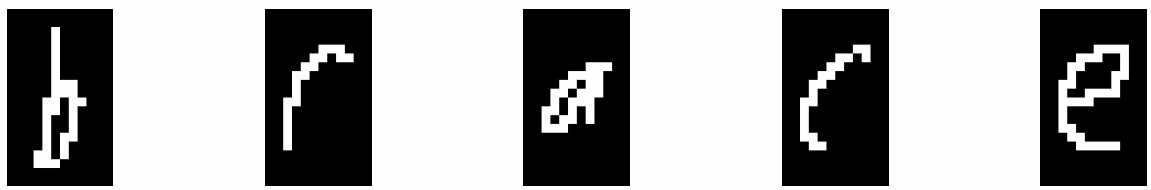
\includegraphics[width=9cm]{brace.jpg}
		\vspace{0.6em}
		\caption{Example word image}\label{fig:brace}
	\end{minipage}
	~~~
	\begin{minipage}[b]{0.33\textwidth}
		\centering 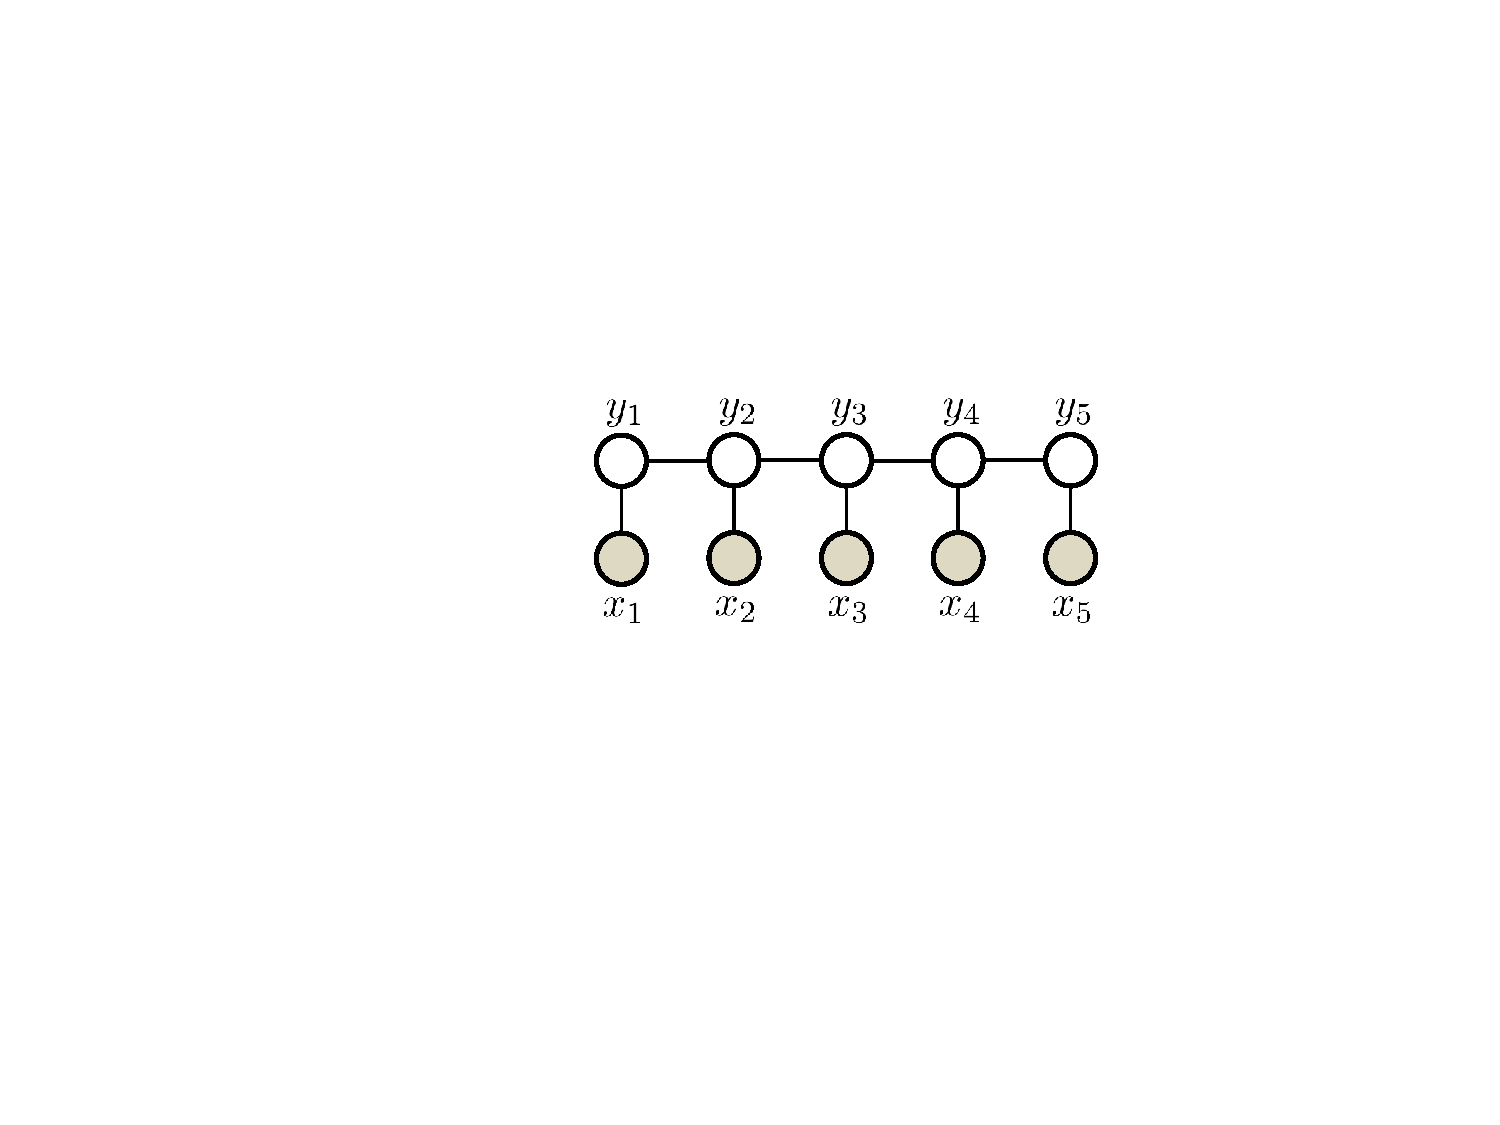
\includegraphics[width=5cm]{crf}
		\caption{CRF for word-letter}\label{fig:CRF_model}
	\end{minipage}
\end{figure}

\paragraph{Conditional Random Fields.}
\label{sec:Condtional_Random_Fields}

The CRF model is the same as what was defined in Assignment 2. However, there is
a difference in the input that is passed to the CRF model. To recall the details
of the OCR dataset - the training set consists of $n$ words. The image of the
$t$-th word can be represented as $X^t = (\xvec^t_1, \ldots, \xvec^t_m)'$, where
$'$ means transpose, $t$ is a superscript (not exponent), and each \emph{row} of
$X^t$ (\eg\ $\xvec^t_m$) represents a letter. Here $m$ is the number of letters
in the word, and $\xvec^t_j$ is a 128 dimensional vector that represents its
$j$-th letter image. To ease notation, we simply assume all words have $m$
letters. The sequence label of a word is encoded as $\yvec^t = (y^t_1, \ldots,
y^t_m)$, where $y^t_k \in \Ycal := \{1, 2, \ldots, 26\}$ represents the label of
the $k$-th letter. So in Figure \ref{fig:brace}, $y^t_1 = 2$, $y^t_2 = 18$,
\ldots, $y^t_5 = 5$.

In this assignment, the CRF model will instead take \emph{convolutional
  features}, given by a function $g$, which you will implement. The details of
the convolution operation is given in Section \ref{par:Convolution}.

Using this (new) notation, the Conditional Random Field (CRF) model for this
task is a sequence shown in Figure \ref{fig:CRF_model}, and the probabilistic
model for a word/label pair $(X, \yvec)$ can be written as
%
\begin{align}
  \label{eq:crf}
  p(\yvec | X ) &= \frac{1}{Z_X} \exp \rbr{\sum_{s=1}^m \inner{\wvec_{y_s}}{g(\xvec_s)} + \sum_{s=1}^{m-1} T_{y_s, y_{s+1}}} \\
  \where Z_X &= \sum_{\hat{\yvec} \in \Ycal^m} \exp \rbr{\sum_{s=1}^m \inner{\wvec_{\yhat_s}}{g(\xvec_s)} + \sum_{s=1}^{m-1} T_{\yhat_s, \yhat_{s+1}}}.
\end{align}
	%
% $Z(X)$ is a normalization constant depending on $X$.
$\inner{\cdot}{\cdot}$ denotes inner product between vectors. Two groups of
parameters are used here:

\vspace{-1em}
\begin{itemize}

\item {\bf Node weight:} Letter-wise discriminant weight vector $\wvec_k \in
  \RR^{128}$ for each possible letter label $k \in \Ycal$;

\item {\bf Edge weight:} Transition weight matrix $T$ which is sized
  $26$-by-$26$. $T_{ij}$ is the weight associated with the letter pair of the
  $i$-th and $j$-th letter in the alphabet. For example $T_{1,9}$ is the weight
  for pair (`a', `i'), and $T_{24,2}$ is for the pair (`x', `b'). In general $T$
  is not symmetric, \ie\ $T_{ij} \neq T_{ji}$, or written as $T' \neq T$ where
  $T'$ is the transpose of $T$.
\end{itemize}

Given these parameters (\eg\ by learning from data), the model \eqref{eq:crf}
can be used to predict the sequence label (\ie\ word) for a new word image $X^*
:= (\xvec^*_1, \ldots, \xvec^*_m)'$ via the so-called maximum a-posteriori (MAP)
inference:
%
\begin{align}
	\label{eq:crf_decode}
	\yvec^* = \argmax_{\yvec \in \Ycal^m} p(\yvec | X^*)
	= \argmax_{\yvec \in \Ycal^m} \cbr{ \sum_{j=1}^m \inner{\wvec_{y_j}}{g(\xvec^*)_j} + \sum_{j=1}^{m-1} T_{y_j, y_{j+1}}}.
\end{align}

When CRF is used as a layer, we need to compute the gradient with respect to its input.
In \eqref{eq:crf}, let us denote $z_s = g(\xvec_s)$. 
Then
\begin{align}
	\nabla_{z_s} p(\mathbf{y}|X) 
	&= \mathbf{w}_{y_s} - \sum_{\hat{\mathbf{y}} \in \mathcal{Y}^m} \frac{\exp(...)}{Z} \cdot \nabla_{z_s} \sum_{s = 1}^m \langle \mathbf{w}_{\hat{y}_s}, z_s \rangle \\
	&= \mathbf{w}_{y_s} -\sum_{\hat{\mathbf{y}} \in \mathcal{Y}^m} p(\hat{\mathbf{y}}|X) \mathbf{w}_{\hat{y}_s} \\
	&= \mathbf{w}_{y_s} - \sum_{\hat{y} \in \mathcal{Y}} p(y_s = \hat{y} |X ) \mathbf{w}_{\hat{y}}.
\end{align}


\section{PyTorch}
\label{sec:PyTorch}
You will use the popular PyTorch deep learning framework to implement all the
algorithms in this assignment. For a comprehensive introduction to PyTorch
please refer to this link
\href{https://pytorch.org/tutorials/beginner/pytorch_with_examples.html}{PyTorch
  Tutorial}.

The above tutorial is a beginner-friendly introduction to the basic concepts of
PyTorch. You will need to be comfortable with all the concepts in that link to
successfully complete this assignment. In particular, pay attention to the
\texttt{nn.module} class. This is a standard way computational units are
programmed in PyTorch. You will implement the \texttt{CRF} layer and the
\texttt{Conv} layer, in the code, as a subclass of the \texttt{nn.module} class.
Refer to the starter code for more details.

Like in the last assignment, Torch has a gradient checker. 
You could use it like this:

https://discuss.pytorch.org/t/how-to-check-the-gradients-of-custom-implemented-loss-function/8546

\section{(20 points) Convolution}

Different from the previous assignment, we are going to feed in convolutional
features of the input image of a letter to the CRF model. Your task is to
\textbf{implement the convolution layer in PyTorch}. Note that PyTorch
implements its own convolution layer (\texttt{nn.conv2d}). You are required to
provide your own implementation and \textbf{NOT} use PyTorch's implementation.
However, you may use PyTorch's implementation of convolution as a reference to
check the correctness of your implementation.

\paragraph{Convolution operation.} \label{par:question1}
\label{par:Convolution}

Convolution is a commonly used image processing technique, applying various
types of transformations on an image. Convolutional Neural Networks (CNNs)
employ multiple layers of convolutions to capture fine-grained image features,
which are further used downstream in learning several computer vision tasks such
as object detection, segmentation etc.

A convolution operation takes in an image matrix $X$ and a filter matrix $K$ and
computes the following function as detailed in Eq 9.6 of [GBC]:
%
\begin{equation}
  \label{eq:conv}
  \hat{X}(i,j) = \sum_{k,l} X(i + k, j+l) K(k,l).
\end{equation}
In our case, the output channel from CNN is 1.
Kernel is square: $5 \times 5$ or $3 \times 3$.

%
\begin{itemize}
\item[(3a)] \textbf{(20 points)} Implement the \texttt{Conv} layer and the
\texttt{get\_conv\_features(x)} function, in the starter code. Once
convolution is implemented, the CRF's \texttt{forward} pass and \texttt{loss}
functions use the convolution features as inputs (the code for this is set up
already).

Your implementation also needs to accommodate different strides,
along with an option of zero padding or not.

\textbf{Testing your implementation.} Your implementation of the {\tt Conv}
layer will contain the implementation of the convolution operation.
%(similar to \tt nn.functional.conv2d} of PyTorch). 
It is crucial to get the implementation
of the convolution operation correct first. Consider this simple example of an
input matrix $X$ and filter matrix $K$, with unit stride and zero padding.
Report the result of convolving the $X$ with $K$. You must write this as a test
case for the grader to run.
%
\[
X = \begin{bmatrix}
1 & 1 & 1 & 0 & 0 \\
0 & 1 & 1 & 1 & 0\\
0 & 0 & 1 & 1 & 1\\
0 & 0 & 1 & 1 & 0\\
0 & 1 & 1 & 0 & 0
\end{bmatrix} ; \quad
K = \begin{bmatrix}
1 & 0 & 1 \\
0 & 1 & 0 \\
1 & 0 & 1
\end{bmatrix}
\]

Implement your test case inside a file {\tt conv\_test.py}. It should run
as a standalone test (with all the dependencies, imports in place),
and print the result on the screen.

{\bf Note.} In PyTorch input to conv2d are \(4\)-D tensors - {(\tt batch\_size
	$\times$ channel\_size $\times$ height $\times$ weight)} for both the input
image $X$ and the filter $K$. In our dataset, we use a single channel input
({\tt channel\_size = 1}).


\fbox{\begin{minipage}{0.93\textwidth}
You only need to implement the forward pass of the convolution layer. There is no need to implement the derivatives. You can use PyTorch's auto-differentiation feature to automatically get backpropagation.
\end{minipage}
}

Having the \verb#backward#() function implemented is an indication to PyTorch that the backward pass is indeed implemented. If a layer in the model is specified to have the \verb#backward# function, then PyTorch will just use it.
Otherwise, if some layers do not have the \verb#backward# function explicitly implemented,
then PyTorch will use autograd to compute the gradients.

\end{itemize}

\section{(50 points) CRF}

Now, you will (re)-implement the CRF model in PyTorch. Note that this version is
designed to use convolutional features and NOT the raw pixels to the CRF model
(recall in Assignment 2 we used raw images pixels as the input features
$\xvec^{t}_{j}$ which is a 128 dimensional vector). Here, they will be replaced
by convolutional features. However, the CRF implementation should remain almost
the same; except for changes in the input and output shapes and the fact that it
needs to be implemented as a layer (\texttt{nn.module}) in PyTorch.

The CRF model is implemented as a \texttt{class} in the \texttt{crf.py} file in
the provided starter code.
%
\begin{itemize}
\item[(4a)] Implement the forward, backward pass and loss inside
  \texttt{crf.py}. This would amount to 
  \begin{enumerate}
  	\item re-implementing the \emph{inference} procedure using dynamic programming (decoder) 
  	\item dynamic programming algorithm for \emph{gradient computation} including with respect to CRF input, $T$, and $w_y$,
  	\item loss - which is the negative log-likelihood of the CRF objective. 
  \end{enumerate} 
	\textbf{You can directly copy from the reference solutions for the last assignment or use your own implementation.}
  Once again, place holders for
  all these are provided in the starter code (in the \texttt{crf.py} file). This
  question will be graded through the subsequent questions.

\item[(4b)] \textbf{(20 points)} Implement and display performance measures on
  the CRF model - we will use the same performance measures as the previous
  assignment (1) \textbf{letter-wise prediction accuracy}, (2) \textbf{word-wise
    prediction accuracy}. Using a batch size of \(64\) plot the letter-wise and
  word-wise prediction accuracies on both training and test data over \(100\)
  iterations (\(x\) axis). (Place holder provided in the startup code). Use a
  \(5 \times 5\) filter matrix for this experiment, and set stride and zero/no
  padding to optimize the test performance.
  Initialize the filters randomly.
  If it has not converged (function value changes little), you may increase the number of iterations.

{\bf Note.} Your model should process the input data batch after batch, therefore the input dimension to your model is 256*14*128 (\verb#batch_size# * \verb#max_word_length# * \verb#num_of_pixels#). The output dimension of the CNN layer (i.e., the input dimension of the CRF layer) should be 256*14*64, where 64 is the length of the features of one letter.

{\bf Note.} In the backward function of CRF, should we calculate and return the gradient of loss with respected to the whole batch of input, which is of dimension 256*14*64? We are calculating the gradient of loss with respect to weights.  But the loss is calculated using the features and not the image itself.

{\bf Note.} You have to make sure that invalid letters do not add any value to your loss function. Moreover, while you are calculating the gradient, you have zero-out the gradients of invalid letters. You cannot just use the true labels to find valid letters because, in test time, the labels are not provided to the model. The solution was to use the input image and find valid images (any image with at least one non-zero pixel). You can use 'torch.any()' and 'torch.where()' for masking and filtering.

  

\item [(4c)] {\bf (20 points)} It is common to use more than one convolution
  layer in modern deep learning models. Convolution layers typically capture
  local features in an image. Stacked convolutions (multiple layers of
  convolutions put one after the other) help capture higher level features in an
  image that has shown to aid classification significantly. Repeat experiments
  in (4b) with the following convolution layers. Set stride and zero/no padding
  to optimize the test performance.


\begin{enumerate}
	\item A Layer with \(5 \times 5\) filter matrix
	\item A Layer with \(3 \times 3\) filter matrix
\end{enumerate}

{\bf Note.} In \verb#crf.py#, the \verb#get_conv_features#() function is merely a "placeholder" for getting the convolution features for the CRF model. The output shape of the conv layer will vary depending on filter size, padding \& stride. You are supposed to handle that (by zero padding) and make the input tensor to the CRF as a fixed shape, after you get convfeatures inside \verb#get_conv_features#().

{\bf Note.} In \verb#train.py#, \verb#conv_shapes# = [[1,64,128]] is a model parameter that specified the input/embedding shapes. Feel free to ignore this parameter and define your own way of handling the shapes. Here $64$ is the embedding dimension, but if you are having multiple convolution layers (stacked convolution layers), then the shapes of the subsequent layers will be different. \verb#Batch_size# is typically not specified in \verb#conv_shapes# since its not a property of the layer; no matter what shapes you specify, the definition of \verb#batch_size# will not impact them, the shape of any data (input/output) will be something like \verb#batch_size# $\times$ a $\times$ b $\times$ c.


{\bf Note.} In \verb#train.py#, what does \verb#embed_dim# = 64 mean? Typically layers are specified via the input and output dimensions that it produces. Here \verb#input_dim# corresponds to the input dimension that the layer takes in and the \verb#embed_dim# is the size of the embedding (output) that the layer produces. These are merely placeholders, meant to help you consider the input and output shapes while programming the CRF layer (and subsequently the conv layer). If this is confusing for you, feel free to setup your own mechanism to correctly handle input output shapes.
The question asks you to perform convolution with different filter shapes. So one way to handle output shapes correctly is to let your convolution layer automatically infer the output shape, given the input shape and filter size; some pointers:

https://fomoro.com/projects/project/receptive-field-calculator

{\bf Note.} Should we use Sequential to concatenate convolution layer and crf layer, or implement a CRF layer that entangles with a couple of convolution layers? Use Sequential. Pass a conv layer (it could be a stack of sequential conv layers) to CRF and use the \verb#get_conv_features#() method to get the features. This way, we are able to easily determine the valid letters from the input image as well. 


\item [(4d)] {\bf (10 points)} Enable GPU in your implementation. Does it lead
  to significant speedup? You can test on the network in 4c. Make sure your plot
  uses wallclock time as the horizontal axis.
\end{itemize}

\section{(30 points) Comparison with Deep Learning}
\label{sec:Analysis}

Compare your new CRF model, with convolution features, with a convolution based
Deep Neural Network (DNN) model of your choice, also known as Convolutional
Neural Networks (CNN). You are free to design your own DNN model or pick one of
the popular model architectures that have been published. Some popular choices
would be,

\vspace{-0.5em}
\begin{enumerate}
\item VGG \cite{ZisSimZis14}
\item ResNet \cite{SunHeZhaRenetal15a}
\item AlexNet \cite{HinKriSutHin12a}
\item GoogLeNet \cite{SerSzeLiuJiaetal14}
\item LeNet \cite{LecBotBenHaf98}
\end{enumerate}
\vspace{-0.5em}

Since all these methods, except LeNet, require resizing the images from 16x8 to 224x224, you can just consider LeNet.
You can use code from online, and build a blank LeNet and train all weights from scratch.  It shouldn't be hard, and it will not take long.
The input to the CNN model will of course be the original train and test
dataset. None of these methods are composed with a CRF.
You will have to report the following in your report.
%
\begin{itemize}
\item[(5a)] \textbf{(10 points)} If you designed your own DNN model, then report
  the implementation details of it, along with the model architecture, loss
  functions etc. If you picked LeNet, explain each of the
  layers inside it and its purpose for the task at hand. 
  That is, what functions (layers) were useful in the solution to the
  problem. In addition, look into the source code and sketch its structure
  within 150 words.

%	You do not need to try out each of the four architectures to justify.
%	You are free to use which ever model you think fits the task. We only ask for a justification on why you chose the model/architecture, based on the individual virtues. 
	
\item[(5b)] \textbf{(5 points)} Plot the letter-wise and word-wise prediction
  accuracies on both training and test data (\(y\) axis) over \(100\) iterations
  (\(x\) axis) (You might have to implement these). Compare this with your CNN+CRF
  results and report your analysis (which model fared better? and why?). You may
  use the hyperparameter that yields the best performance for your CNN+CRF
  model.
  If it has not converged in 100 iterations, you may increase the number of iterations.
  
  Sometimes, your program might run out of memory. In this case, you will have to adjust the batch size.  This post might help:
  
  \url{https://stats.stackexchange.com/questions/284712/how-does-the-l-bfgs-work}
  
  
  
\item[(5c)] {\bf (5 points)} Change the optimizer from {\em LBFGS} to {\em
    ADAM}. Repeat the experiments in (5b) and report the letter-wise and
  word-wise accuracies, with \(x\)-axis as the \#iterations. Does {\em ADAM} find
  a better solution eventually, and does it converge faster than {\em LBFGS}?


\item[(5d)] \textbf{(10 points)} Why did you choose this model (again it could
  be your own design or an off-the-shelf model)? More precisely you should
  explain every design decision (use of batchnorm layer, dropout layer etc) and
  how it helped in the task at hand, in your report.
\end{itemize}


\bibliography{references} \bibliographystyle{plain}
%\section{Convolutional filters}
\label{sec:appdxconvfilters}



\end{document}
